\documentclass[12pt, openany, oneside, a4paper, english, brazil]{abntex2}   % Padrão Abntex2

%***************************** PACOTES *********************************** %
\usepackage[pdftex]{color,graphicx}

%\usepackage[within=none]{newfloat}
\usepackage[utf8]{inputenc}		     % Codificacao do documento (conversão automática dos acentos)


%	Fonte
\usepackage[T1]{fontenc}		   	 % Selecao de codigos de fonte.
\usepackage[brazil]{babel}
\usepackage{lmodern}			     % Usa a fonte Latin Modern

%	Matemático e Gráfico
\usepackage{float}
\usepackage{graphics,graphicx}	     % pacotes para inserir figuras .eps ou .jpg
\graphicspath{{figuras/}}            % pasta de figuras
\usepackage{amssymb}           		 % pacote para fontes e simbolos matemáticos
\usepackage{longtable}          	 % possibilita inserir grandes tabelas
\usepackage{makecell}                % possibilita pular linhas nas tabelas
\usepackage{xcolor,colortbl,multirow} % permite textos e tabelas com cores
\usepackage{amsmath}           		 % pacote para equações
\usepackage{epstopdf}
\usepackage{ragged2e}
\usepackage{listings}
%\lstset{numbers=left, numberstyle=\tiny, stepnumber=1, numbersep=5pt, basicstyle=\scriptsize ,frame=tbrl}
\usepackage{etoolbox}
\usepackage{multicol}
%\usepackage{caption}
\usepackage[position=b,singlelinecheck=on]{subfig}

\floatstyle{plaintop}
\newfloat{quadro}{htbp}{loq}
\floatname{quadro}{Quadro}

\makeatletter
\patchcmd{\listof}% <cmd>
{\float@listhead}% <search>
{\@namedef{l@#1}{\l@table}\float@listhead}% <replace>
{}{}% <success><failure>
\makeatother

%\makeatletter
%\renewcommand*{\float@listhead}[1]{%
%	\@ifundefined{chapter}{%
%		\section*{#1}%
%		\addcontentsline{toc}{section}{#1}%
%	}{%
%	\chapter*{#1}% 
%	\addcontentsline{toc}{chapter}{#1}%
%}%
%\@mkboth{\MakeUppercase{#1}}{\MakeUppercase{#1}}%
%}
%\makeatother




%\DeclareFloatingEnvironment{quadro}[Quadro][Lista de quadros]
%\DeclareCaptionType{quadro}[Quadros][Lista de quadros]


% % % % % % % % % % % % % % % % % % % %

\definecolor{codegreen}{rgb}{0,0.6,0}
\definecolor{codegray}{rgb}{0.5,0.5,0.5}
\definecolor{codepurple}{rgb}{0.58,0,0.82}
\definecolor{backcolour}{rgb}{0.95,0.95,0.92}

%\definecolor{verde}{rgb}{0,0,0}

\lstdefinestyle{mystyle}{
	backgroundcolor=\color{backcolour},   
	commentstyle=\color{codegreen},
	keywordstyle=\color{magenta},
	numberstyle=\tiny\color{codegray},
	stringstyle=\color{codepurple},
	basicstyle=\footnotesize,
	breakatwhitespace=false,         
	breaklines=true,                 
	captionpos=b,                    
	keepspaces=true,                 
	numbers=left,                    
	numbersep=5pt,                  
	showspaces=false,                
	showstringspaces=false,
	showtabs=false,                  
	tabsize=2
}

\lstset{style=mystyle}

%	Estrutural
\usepackage{url}
\usepackage{threeparttable}     	 % permite a inserção de notas de rodapé nas tabelas
\usepackage{lscape}             	 % orientação de página LANDSCAPE
\usepackage{pifont}             	 % acrescenta símbolos diferentes.
%\usepackage{cmap}					 % Mapear caracteres especiais no PDF	
\usepackage{lastpage}				 % Usado pela Ficha catalográfica
\usepackage{indentfirst}			 % Indenta o primeiro parágrafo de cada sessão.



% Pacotes de citações
\usepackage[brazilian,hyperpageref]{backref}	 % Paginas com as citações na bibl
\usepackage[alf]{abntex2cite}	% Citações padrão ABNT numerica
     
% remover bordas dos links
\hypersetup{
    colorlinks,
    linkcolor={black},
    citecolor={black},
    urlcolor={black}
} % resto dos pacotes Latex
%\usepackage[english]{style/UCSAL-Template} % personalização da ABNTEX2 para escrita em inglês
\usepackage[portuguese]{style/ucsal} % personalização da ABNTEX2 para escrita em português
\usepackage{longtable}
\usepackage{blindtext}
\DisemulatePackage{setspace}
\usepackage{setspace}
\usepackage{lipsum}
\usepackage[left=3cm,top=3cm,right=2cm,bottom=2cm]{geometry}
\usepackage{fontspec}
\setmainfont{Arial}
\usepackage{hyperref}
\usepackage{graphicx}




%inserindo apenas uma página

%---------------------------------------------------------------
%--------- DADOS BÁSICOS DO TRABALHO (Preencher todos) ---------
%---------------------------------------------------------------


\titulo{Ensino de matemática básica: Uma abordagem usando elementos de gamificação com estratégia educacional para crianças com síndrome de down
}   % Título do Trabalho em Português

\tituloingles{Teaching basic mathematics: An approach using gamification elements with an educational strategy for children with down syndrome}   % Título do Trabalho em Inglês

\palavraschave{1. Gamificação.
2. Educação Matemática.
3. Crianças com Síndrome de Down.
4. Aplicativo educacional.}  % 5 palavras-chave

\keywords{1. Gamification.
2. Mathematics Education.
3. Children with Down Syndrome.
4. Educational App.}   % 5 palavras-chave para resumo em inglês

\DEELautor{ Cristiano Filho\\Enzo Santana \\Jamile Conceição\\ Lucas Augusto\\ Vinicius Candeias\\}{} % Alunos autores do trabalho



\curso{Bacharelado em Engenharia de Software}												
\orientador{Flávio Dusse}  % Professor Orientador membro da banca 

\membrob{Prof. Me. Segundo professor}   % Professor membro da banca 
\membroc{Prof. Me. Terceiro professor}   % Professor membro da banca

\local{Salvador}   % Cidade da instituição
\data{2024}        % Ano de realização

%--------------------------------------------------------------------------------------------



\begin{document}
\onehalfspacing

% Seleção automática do idioma, não alterar
\ifx\isenglish\undefined
    \selectlanguage{brazil}
\else
    \selectlanguage{english}
\fi

% Texto da Dedicatória (OBS: dedicatória é opcional)
% Caso não queira inserir, deixe em branco ( \dedicatoria{} )
\DEELdedicatoria{Dedico este trabalho a todos aqueles.... \\}  
    
% Texto dos Agradecimentos (OBS: Agradecimentos é opcional)
% Caso não queira inserir, deixe em branco ( \agradecimentos{} )
\DEELagradecimentos{Eu Cristiano agradeço primeiramente a Jeová Deus e a minha família que sempre me apoiou nessa trajetória com todas as adversidades.} 

                       
% Texto da Epígrafe (OBS: Epígrafe é opcional)
% Caso não queira inserir, deixe em branco ( \epigrafe{} )
\DEELepigrafe{\textit{"A alegria está na luta, na tentativa, no sofrimento envolvido e não na vitória propriamente dita."} \\ (Mahatma Gandhi 
)} 
    

% Texto do Resumo (OBS: Resumo é Obrigatório)
\DEELresumo{
Este trabalho de conclusão de curso tem como objetivo o desenvolvimento de um aplicativo gamificado destinado ao ensino de matemática básica para crianças com Síndrome de Down, com idades entre sete e quinze anos. O aplicativo contará com sessões interativas, desafios cativantes, recompensas motivadoras e feedback imediato, todos projetados para enriquecer a experiência de aprendizado dessas crianças. O diferencial deste projeto é a incorporação de uma interação por voz, permitindo que as crianças respondam às perguntas usando sua própria voz. Essa funcionalidade não apenas melhora as habilidades matemáticas, mas também desempenha um papel crucial no desenvolvimento da linguagem e da comunicação das crianças. Essas melhorias na comunicação têm o potencial de transformar significativamente a vida cotidiana dessas crianças, aumentando sua independência e confiança. Este projeto visa criar uma ferramenta educacional inclusiva e estimulante, que não apenas promova o aprendizado da matemática, mas também proporciona uma melhora na dicção e portanto na interação social das crianças com Síndrome de Down.} 
     
% Texto do Abstract (OBS: Abstract é Obrigatório)
\DEELabstract{
This undergraduate thesis aims to develop a gamified application designed for teaching basic mathematics to children with Down syndrome, aged between seven and fifteen years old. The application will feature interactive sessions, engaging challenges, motivating rewards, and immediate feedback, all designed to enrich the learning experience for these children. The unique aspect of this project is the incorporation of voice interaction, allowing children to respond to questions using their own voices. This functionality not only enhances mathematical skills but also plays a crucial role in language and speech development for these children. These improvements in communication have the potential to significantly transform the daily lives of these children, increasing their independence and confidence. This project aims to create an inclusive and stimulating educational tool that not only promotes mathematics learning but also provides valuable benefits for the communication and social interaction of children with Down syndrome.} 
    



%%%%%%%%%%%%%%%%%%%%%%%%%%%
%% Elementos Pré-Textuais%%
%%%%%%%%%%%%%%%%%%%%%%%%%%%
\ElementosPreTextuais
% Insere todos os elementos Pré-Textuais listados (capa, folha de rosto, ...)
    % capa                   % Obrigatório
    % folhaderosto           % Obrigatório
    % folhaaprovacao         % Obrigatório
	% dedicatoria            % Opcional
	% agradecimentos         % Opcional
    % epigrafe               % Opcional
    % resumo                 % Obrigatório
    % abstract               % Obrigatório

%\newpage
%--------Lista de figuras--------
\ListaDeFiguras 
%--------Lista de tabelas--------
\ListaDeTabelas 
%--------Lista de Siglas e Abreviaturas--------
%----------Lista de Acronimos --------------------------------
\ifx\isenglish\undefined
\pretextualchapter{Lista de Siglas e Abreviaturas}
\else
\pretextualchapter{Acronyms}
\fi


%\renewcommand{\baselinestretch}{2} %espaçamento entre linhas (por definicçào, no espABNT é 2)
\begin{tabbing}
xxxxxxxxxxx \= xxxxxxxxxxxxx \kill
\textsc{API}            \> \textit{Application Programming Interface}\\

\textsc{BES}            \> \textit{Bacharelado em Engenharia de Software}\\

\textsc{RF}             \> \textit{Requisitos Funcionais}\\

\textsc{RNF}            \> \textit{Requisitos Não Funcionais}\\

\textsc{RN}            \> \textit{Regra de Negócio}\\

\textsc{MVP}            \> \textit{Mínimo Produto Viável}


\end{tabbing}

%\addcontentsline{toc}{chapter}{Lista de Siglas e Abreviaturas}
   
%--------Lista de Simbolos e Notação--------
%\include{list_simbolos} 
%--------Sumário-------
\Sumario


%%%%%%%%%%%%%%%%%%%%%%
%%Elementos Textuais%%
%%%%%%%%%%%%%%%%%%%%%%
\textual 
\chapter{Introdução}\label{chp:intro}

Em síntese, refletir de forma lúdica e interativa, pode estabelecer uma conexão com os alunos interligados à matemática. Se fez necessário a criação de uma ideologia de  aplicação representado por um personagem chamado Polvo Pi, desenvolvido para conduzir e motivar principalmente o público infantil e interessados no aprendizado através da aplicação educativa. A missão principal do persona é ajudar o colegiado do Ensino Fundamental I, trazendo vínculos e identificações por parte dos estudantes, despertando a descobrirem como a matemática pode ser divertida e fascinante, utilizando jogos, desafios e histórias envolventes para ensinar conceitos matemáticos de maneira simples, conduzindo a imersão em um novo mundo numa troca constante de conhecimento. \cite{Lopes2020}

Math.Pow acredita que as dificuldades enfrentadas no ensino da matemática podem ser superadas com o auxílio da tecnologia como ferramenta, bastando encontrar a maneira certa de aprender. A aplicação tem como principal objetivo viabilizar a elaboração de metodologias de ensino através de planejamentos pedagógicos eficientes e criativos. A escolha do melhor nome para representar essa nova ferramenta, está coerente a fatores científicos, relações e comparações. Sendo assim o nome escolhido é “Math.Pow”:

POLVO: é um animal marinho de corpo mole e flexível, possuindo oito braços chamados tentáculos, conhecido por sua inteligência, habilidades de camuflagem e comportamentos complexos; ele serve como inspiração para a idealização da aplicação educativa. Da família dos cefalópodes, este molusco busca se adaptar a uma variedade de ambientes para sobreviver. Por analogia, sob o mesmo ponto de vista. Do mesmo modo, a ideia em forma de aplicação se adapta às diferentes maneiras de aprendizado dos alunos, utilizando as características-chave desse fascinante mamífero pelágico almejando tornar o ensino mais eficaz e envolvente.\cite{BBC2023}




\section{Aplicabilidade e Motivação}\label{chp:aplic}

A dificuldade encontrada na docência do Ensino Fundamental I nas atribuições das aulas de matemática, tratam-se de abordagens que proporcionam alternâncias e intercorrências consideráveis. Os problemas, contratempos e adversidades apresentam-se desde os planejamentos pedagógicos por coordenadores em planos de cursos e sobrevêm chegando até os docentes em seus planos de aulas que não conseguem atingir com eficiência o entendimento e absorção da aprendizagem pelos discentes. 

Tanto o magistério quanto o alunato enfrentam objeções ao lidar com essa disciplina, procurando superar muitos obstáculos, ponderando que os incentivos deparam em grande parte dos estudantes que não consideram a matemática como algo notável ou concebível em suas vivências. Além disso, os estímulos para aprendizagem, aplicação das suas concepções e ideias são diretamente impactados. Igualmente a subjetividade e complexidão da matemática abrange concepções subjetivas e constantemente abstrusa, existindo a possibilidade do alunado encontrar obstruções para perceber e assimilar os conceitos, o que pode trazer o desapontamento. 

Da mesma forma a fixação e cognição dos estudantes focalizam em memorar os métodos e suas fórmulas em vez de tentar compreender os princípios implícitos subentendidos, impossibilitando a sua criatividade para solucionar determinadas questões com eficacia. Assim também as ferramentas necessárias para os educadores deparam-se com impedimentos para obter materiais instrutivos, compatíveis e metodologias de transmissão de conhecimentos eficientes, considerando a probabilidade de impactos negativos na natureza da orientação. Por analogia a aflição pela disciplina é perceptível em grande parte dos alunos que se apresentam ansiosos, pois o processo de aprender matemática oferece tendências que afetam a conduta e autoestima. 

Atualmente a maior parte dos jovens e até mesmo alguns adultos vivenciam a sensação de experienciar jogos com parâmetros físicos ou digitais por intermédio de videogames, computadores, smartphones, dominós, baralhos, dados etc. Subsiste neles alguma coisa indeterminada que atrai e magnetiza, tomando por completo a atenção do usuário. Que idealiza a sobrelevação, individualmente ou em equipe, incentivado com o resultado alcançado em suas fases, etapas, níveis e etc. Pois mesmo parecendo uma simples diversão, nas variadas formas e possibilidades de jogos se aplica energia espontaneamente. Além disso as atividades de entretenimentos, define a estruturação intrínseca mediante a diretrizes que tem por objetivo conduzir a atividade com procedimentos organizados.

\section{Contextualização}

A gamificação, que utiliza elementos de jogos para engajar e motivar os alunos, tem se destacado como uma abordagem eficaz para o ensino. A gamificação oferece oportunidades de aprendizado interativo, onde desafios, recompensas e feedbacks imediatos podem tornar a experiência educacional mais estimulante e atraente para as crianças.

A evolução das tecnologias tem facilitado significativamente a inclusão de pessoas com deficiência, proporcionando maior acessibilidade e autonomia. Novos recursos e APIs que facilitam a interconexão e integração entre plataformas, têm possibilitado o desenvolvimento de aplicações e soluções tecnológicas que atendam a um número cada vez maior de usuários com necessidades especiais. Um exemplo disso é o aplicativo "Hand Talk", que disponibiliza um plugin para integrações de acessibilidade a deficientes auditivos, permitindo tradução automática para Língua Brasileira de Sinais.

Outras iniciativas importantes são ferramentas de leitura de tela, ampliação de conteúdo, contraste elevado e interfaces adaptáveis. Essas inovações têm o poder de reduzir barreiras, promover inclusão digital e transformar positivamente a vida de pessoas com deficiência. Como destaca  \cite{furlan2016desenvolvimento}, "a tecnologia tem um papel crucial na promoção da acessibilidade e inclusão das pessoas com deficiência".


\section{Objetivos}

Afinal de contas, qual é a definição de gamificação? Quais são os pontos de uniformidade, divergência e convergência entre gamificação e jogos? Como pôr em prática? Neste estudo acadêmico, a abordagem da gamificação será abrangente, com reflexões e idealizações que se referem a um tema atual que estabelece relações de grande importância no âmbito da educação.O elemento conceitual investigativo deste objeto de pesquisa é muito significativo, dado que a gamificação requer um entendimento satisfatório para ser empregue com eficiência, sensatez e seriedade. A temática será abordada em tópicos considerados relevantes. Investigando as concepções e ideias empregadas, os recursos e componentes adotados, referenciando determinadas finalidades. Destarte, busca-se obter um entendimento referente ao conteúdo discutido neste trabalho de pesquisa e investigação científica, considerando que esta abordagem dissertada se trata de uma esfera que denota grande relevância mostrando considerável importância no campo acadêmico.


\subsection{Objetivo Geral}

 O principal objetivo desse trabalho de conclusão de curso é analisar o uso da gamificação através de um aplicativo,  enquanto uma metodologia ativa , para o ensino de matemática, com  alunos do fundamental I. Como ferramenta para auxílio na pesquisa temos como objetivo inicial a produção um aplicativo que usa elementos de gamificação, a escolha de um aplicativo é que não tenha a necessidade de ser usado somente em sala de aula, e sim para servir como ferramenta auxiliar no processo de ensino.


\subsection{Objetivos Específicos}

\begin{itemize}
\item{Autenticar se o uso de jogos educacionais para o ensino de matemática é eficaz.
}
\item {Avaliar quais conteúdos são mais estruturantes para o ensino da matemática no fundamental I.
} 
\item {Desenvolver sequências didáticas com a metodologia da gamificação.
 }  
\item {Desenvolver um aplicativo com uso das técnicas de gamificação.
}
\item {Validar o uso do aplicativo com professores e estudantes.
}
\item {Auxiliar no ensino de matemática para alunos do ensino fundamental I.
}
\end{itemize}

\section{Estrutura do Trabalho}

No Capítulo 1 é apresentado o objetivo geral e objetivos específicos, enquanto que o Capítulo 2 traz a Fundamentação Teórica. No Capítulo 3 está apresentada a metodologia do trabalho, enquanto que no Capítulo 4 são apresentados o experimento e coleta de dados. Finalmente, no Capítulo 5 é apresentada a conclusão desta monografia.


 % Texto do cap1.tex
\chapter{Fundamentação Teórica}\label{chp:rev}
\section{Ensino e Aprendizagem}

A aprendizagem é um processo que envolve a interação entre o professor e o aluno, sendo o papel do professor central para que o ensino seja eficaz. Conforme mencionado por \cite{DubetMartucelli1996}, o sistema escolar deve cumprir duas funções fundamentais: a construção de um indivíduo autônomo, capaz de refletir e se autorregular, e a socialização, que promove a integração de normas e valores sociais. Nesse sentido, a escola se torna um ambiente que perpetua a experiência humana como cultura, conforme destaca \cite{Forquin1992}.

A concepção construtivista, segundo \cite{Scheerens2004}, enfatiza a interdependência entre ensino e aprendizagem, tratando-os como processos inseparáveis. Nesse modelo, a aprendizagem é definida como “um processo de construção de significados e atribuição de sentido”, enquanto o ensino consiste na “ajuda necessária para que esse processo se realize na direção desejada”. Essa ajuda deve ser ajustada às necessidades e características do aluno, promovendo desafios acessíveis e que estimulem a reconstrução dos conhecimentos prévios, como argumentado por \cite{MarchesiMartin2003}.

Ainda sobre as práticas do professor, \cite{Onrubia1993}, citado em \cite{MarchesiMartin2003}, ressalta que a ajuda educativa só será eficaz se for capaz de mobilizar os esquemas de conhecimento do aluno e forçar sua reestruturação. Isso implica oferecer um ensino que se conecte diretamente à realidade e ao contexto dos estudantes, promovendo um aprendizado significativo.

O modelo QAIT, proposto por \cite{Slavin1986}, destaca que quatro elementos são essenciais para um ensino eficaz: qualidade da instrução, adequação ao nível dos alunos, incentivo à aprendizagem e tempo suficiente para absorção do conteúdo. Esses elementos devem estar integrados para garantir a eficácia do processo de ensino-aprendizagem.

Por outro lado, a perspectiva afetiva do professor também é essencial. Segundo \cite{FukudaPasquali2002}, aspectos como empatia, relacionamento positivo com os alunos e motivação são cruciais para estabelecer um ambiente de aprendizado efetivo. Esses elementos são complementados por características técnicas, como o domínio do conteúdo e a clareza na comunicação, conforme discutido por \cite{Silva1992}.

Em suma, a eficácia do ensino está diretamente relacionada à capacidade do professor de equilibrar habilidades técnicas e afetivas, adaptando suas estratégias às necessidades dos alunos e promovendo um ambiente de aprendizado inclusivo e motivador. Como destacam \cite{RosenshineStevens1986}, a interação entre práticas instrutivas bem planejadas e a adaptação ao ritmo dos estudantes é fundamental para garantir o sucesso educacional.

O ensino é um processo complexo que envolve tanto habilidades técnicas quanto interpessoais, sendo essencial para promover a aprendizagem e o desenvolvimento dos estudantes. Segundo \cite{DubetMartucelli1996}, o ensino eficaz deve desempenhar duas funções fundamentais: formar indivíduos autônomos, capazes de analisar e regular suas próprias ações, e promover a socialização, integrando normas, valores e conhecimentos que os preparem para participar ativamente na sociedade.

No contexto pedagógico, a eficácia do ensino depende de uma combinação de fatores. \cite{Scheerens2004} ressalta que o ensino deve ser entendido como um suporte contínuo para a construção de significados pelos alunos. Essa perspectiva destaca a importância da interação entre professor e aluno, considerando que a qualidade do ensino está diretamente relacionada à capacidade do professor de ajustar suas estratégias às necessidades de aprendizagem.

A prática pedagógica também se beneficia de modelos teóricos, como o modelo de ensino eficaz proposto por \cite{Slavin1986}. O modelo QAIT enfatiza quatro elementos essenciais: qualidade da instrução, adequação do nível de ensino, incentivo e tempo. Esses fatores, segundo o autor, precisam ser integrados e adaptados ao contexto para que o ensino produza os resultados esperados.

Além disso, a literatura destaca a importância de práticas pedagógicas baseadas em princípios reguladores. \cite{BrophyGood1986} argumentam que estratégias como o uso de reforços positivos, a interação ativa entre professor e alunos e a clareza na organização das aulas são fundamentais para a eficácia do ensino. Essas práticas, ao serem aplicadas, facilitam o aprendizado e promovem o desenvolvimento de habilidades cognitivas e emocionais.

Outro ponto relevante é o papel do professor na mediação do conhecimento. Conforme \cite{MarchesiMartin2003}, o professor eficaz não apenas transmite conteúdos, mas também ajuda os alunos a conectar novos conhecimentos com os já existentes. Essa abordagem reflete o ensino como um processo dinâmico e adaptativo, no qual o professor atua como facilitador da aprendizagem.

Por fim, \cite{RosenshineStevens1986} apontam que estratégias como a revisão do conteúdo, prática supervisionada e feedback contínuo são elementos chave para o ensino eficaz. Essas práticas permitem que os alunos consolidem o aprendizado de forma progressiva, garantindo a retenção e a aplicação prática dos conhecimentos adquiridos.

Em suma, o ensino eficaz é caracterizado por uma interação equilibrada entre planejamento, comunicação, motivação e adaptação às necessidades dos alunos. Essa abordagem, conforme os autores destacados, é essencial para promover o sucesso acadêmico e o desenvolvimento integral dos estudantes.

Entende-se que os métodos de ensino e de aprendizagem são expressões educacionais e, ao mesmo tempo, uma resposta pedagógica às necessidades de apropriação sistematizada do conhecimento científico em um dado momento histórico representando um processo dialético de produção \cite{lacanallo2007metodos}.

\section{Modelos de Ensino}
No processo de ensino-aprendizagem existem diferentes modelos de ensino que os professores podem utilizar para repassar o conteúdo da disciplina e a sua bagagem de conhecimento a respeito do assunto para os alunos \cite{kruger2013metodo}. Nesta seção, apresentamos um panorama dos principais modelos de ensino, explorando suas características e potencialidades, buscamos criar um contexto para a análise da gamificação, evidenciando como essa abordagem pode se integrar e complementar as práticas pedagógicas existentes, com o objetivo de tornar o aprendizado da matemática mais envolvente, significativo e eficaz para os alunos.

\subsection{Ensino Tradicional}

O ensino tradicional, enraizado na história da educação, é caracterizado pela centralização do professor como figura de autoridade e transmissor de conhecimento \cite{kruger2013metodo}. Segundo \cite{mezzari2011}, nessa abordagem o aluno assume um papel passivo, recebendo informações de forma estruturada e com ênfase na memorização de conteúdos . As aulas expositivas, nas quais o professor apresenta o conteúdo de forma oral, são uma das principais metodologias utilizadas nesse método \cite{weintraub2011}.

No ensino tradicional, o professor define o conteúdo programático, a organização das aulas e as atividades a serem realizadas pelos alunos \cite{santos2011}. A ênfase está na reprodução do conhecimento transmitido pelo professor, muitas vezes por meio de exercícios e atividades que visam a fixação do conteúdo \cite{pinho2010}.

Embora o método tradicional seja criticado por sua falta de flexibilidade e por não estimular a autonomia e o pensamento crítico dos alunos \cite{backes2010}, ele ainda é amplamente utilizado em diversos contextos educacionais \cite{teofilo2009}. Alguns autores defendem que o método tradicional pode ser eficaz em determinadas situações, como no ensino de conceitos básicos e na transmissão de informações de forma clara e concisa \cite{oliveira2012}. No entanto, a crítica predominante é que esse método não favorece o desenvolvimento de habilidades como a resolução de problemas, a criatividade e o pensamento crítico, que são cada vez mais importantes no mundo atual \cite{haddadetal1993}.

\subsection{Construtivismo}
O construtivismo, baseado nas teorias de Piaget e Vygotsky, é um método de ensino que coloca o aluno como protagonista no processo de aprendizagem \cite{coria-sabini2003,gomesbellini2009}. Nessa abordagem, o professor atua como facilitador, incentivando a construção do conhecimento por meio da interação do aluno com o ambiente e com os outros \cite{haddadetal1993}. O aluno é encorajado a descobrir o conteúdo por meio de pesquisas e atividades que promovam a reflexão e a compreensão \cite{coria-sabini2003}.

No método construtivista, o professor não é mais o detentor absoluto do conhecimento, mas sim um guia que auxilia o aluno a desenvolver suas próprias ideias e conclusões \cite{coria-sabini2003}. A ênfase está no aprendizado ativo, na experimentação e na resolução de problemas, buscando estimular a autonomia e o pensamento crítico dos alunos \cite{pinho2010}.

Uma das vantagens do método construtivista é a possibilidade de utilizar diversas fontes de informação, como livros, internet e outros recursos, para enriquecer o processo de aprendizagem \cite{chahuanjimenez2009}. Além disso, o trabalho em grupo é valorizado como forma de promover a colaboração, a troca de ideias e o desenvolvimento de habilidades sociais \cite{cogo2006}.

Apesar de suas potencialidades, o método construtivista também apresenta desafios, como a dificuldade do professor em conduzir uma turma com diferentes ritmos de aprendizagem e a necessidade de um planejamento cuidadoso das atividades para garantir que os alunos alcancem os objetivos de aprendizagem \cite{haddadetal1993,pinho2010}.

Dentro do modelo construtivista, diversas metodologias de ensino se destacam, como a Aprendizagem Baseada em Projetos, a Sala de Aula Invertida e a Gamificação, entre outras. Estas serão exploradas nas próximas seções.

\subsubsection{Aprendizagem Baseada em Projetos}

A Aprendizagem Baseada em Projetos (ABP) é uma metodologia ativa que se destaca por sua abordagem dinâmica e centrada no aluno \cite{alecia2022}. Em contraste com as metodologias tradicionais, nas quais o professor assume o papel central de transmissor de conhecimento, a ABP coloca o aluno como protagonista do processo de aprendizagem \cite{fartura2007}.

Na ABP, os alunos são desafiados a investigar e solucionar problemas reais e relevantes para o seu contexto, o que estimula o desenvolvimento de habilidades como pensamento crítico, colaboração, comunicação e autonomia \cite{moran2014}. Ao longo do projeto, os alunos se envolvem em atividades práticas, pesquisas, experimentos e discussões, construindo o conhecimento de forma ativa e significativa.

Um dos pontos fortes da ABP é a sua flexibilidade e adaptabilidade a diferentes áreas do conhecimento e níveis de ensino \cite{bacich2018}. No contexto do ensino de química, por exemplo, a ABP pode ser utilizada para explorar temas como sustentabilidade, meio ambiente, saúde e tecnologia, tornando o aprendizado mais relevante e conectado à realidade dos alunos.

Para que a ABP seja implementada com sucesso, é fundamental que os professores estejam preparados para assumir o papel de mediadores e facilitadores do processo de aprendizagem \cite{diesel2017}. Isso implica em planejar e estruturar o projeto de forma clara, definir objetivos de aprendizagem significativos, selecionar recursos adequados e acompanhar o progresso dos alunos de forma individualizada.

Em suma, a Aprendizagem Baseada em Projetos (ABP) representa uma abordagem pedagógica inovadora e promissora, capaz de transformar a forma como os alunos aprendem e se envolvem com o conhecimento \cite{arthur2020}. Ao adotar a ABP, os professores podem criar experiências de aprendizagem mais engajadoras, significativas e relevantes para os alunos, preparando-os para os desafios do século XXI.

\subsubsection{Sala de Aula Invertida}

A Sala de Aula Invertida (SAI) é uma metodologia ativa de ensino e aprendizagem que propõe uma inversão do modelo tradicional. O estudo do conteúdo conceitual, tipicamente realizado em sala de aula, passa a ser feito em casa pelo aluno, enquanto as atividades reflexivas e de resolução de dúvidas, geralmente feitas em casa, são transferidas para a sala de aula \cite{Bergmann_2016}.

\cite{Pavanelo_2017} diz que essa inversão tem como objetivo central tornar o aluno protagonista do seu processo de aprendizagem, incentivando a autonomia e a responsabilidade. Ao estudar o conteúdo previamente, o aluno chega à sala de aula com uma base de conhecimento, permitindo que o tempo em sala seja dedicado à discussão, resolução de dúvidas e atividades práticas, com o professor atuando como mediador e facilitador .

De acordo com \cite{Pavanelo_2017} a (SAI) se mostra particularmente relevante no contexto atual, em que as tecnologias digitais estão cada vez mais presentes na vida dos alunos. A flexibilidade de horários e a personalização do ensino, características dessa metodologia, atendem às necessidades dos estudantes que estão constantemente conectados ao mundo virtual .

Pesquisas indicam que a SAI pode ser aplicada com sucesso em diversas etapas da Educação Básica, desde os anos iniciais do Ensino Fundamental até o Ensino Médio, promovendo maior participação dos alunos e aprendizagem significativa \cite{Muraro_2019,Sanches_2019}.

Segundo \cite{Bergmann_2016} algumas das vantagens da SAI, incluem :
\begin{itemize}
\item Maior engajamento e responsabilidade do aluno no processo de aprendizagem 
\item Flexibilidade de tempo e personalização do ensino, atendendo às necessidades individuais dos alunos.
\item Otimização do tempo em sala de aula, permitindo que o professor se dedique mais às dúvidas e dificuldades dos alunos.
\item Possibilidade de revisão do conteúdo quantas vezes forem necessárias, com o aluno controlando o ritmo do aprendizado.
\item Fortalecimento da relação professor-aluno e aluno-aluno, por meio de atividades colaborativas e interação em sala de aula.    
\end{itemize}

No entanto, é importante ressaltar que a implementação da SAI exige planejamento e dedicação por parte do professor. A produção de materiais adequados, a escolha de plataformas online e a criação de estratégias para o tempo em sala de aula são alguns dos desafios a serem enfrentados \cite{Rodrigues_2020}.

\subsubsection{Gamificação}

A gamificação, segundo \cite{busarello2014gamificacao}, é a aplicação de elementos de jogos em contextos que não são jogos, como ambientes educacionais. Essa técnica visa aumentar o engajamento e a motivação dos alunos, utilizando elementos como competição, recompensas, desafios e feedbacks instantâneos . No contexto educacional, a gamificação pode tornar o aprendizado mais envolvente e atraente, estimulando a motivação dos estudantes e facilitando o engajamento com o conteúdo \cite{goncalves2021modelo}.

\cite{piaget1993formacao} destaca a importância do jogo no desenvolvimento infantil, argumentando que, ao jogar, a criança desenvolve suas percepções, inteligência e instintos sociais . A gamificação, ao incorporar elementos lúdicos no processo de ensino-aprendizagem, alinha-se com a visão de Piaget sobre a importância do jogo na educação.

\cite{vigotsky2007formacao} também contribui para a compreensão da gamificação na educação . Sua teoria sociocultural enfatiza a importância da interação social na aprendizagem, e a gamificação pode ser uma ferramenta poderosa para promover essa interação. Ao trabalhar em equipe, colaborar e competir em jogos educativos, os alunos desenvolvem habilidades sociais e cognitivas importantes.

A gamificação também se alinha com a teoria de \cite{keller2017development}, conhecida como ARCS (Atenção, Relevância, Confiança e Satisfação) . Essa teoria destaca os elementos necessários para motivar o aluno no processo de aprendizagem. A gamificação, ao utilizar elementos de jogos como desafios, recompensas e feedbacks, pode atender a esses elementos e aumentar a motivação e o engajamento dos alunos.

Outro conceito relevante é o de fluxo, discutido por \cite{hamari2014measuring}. O fluxo é um estado de concentração profunda e envolvimento em uma atividade desafiadora. A gamificação, ao criar atividades desafiadoras e recompensadoras, pode levar os alunos a experimentarem o estado de fluxo, aumentando sua concentração e engajamento no aprendizado.

Em suma, a gamificação é uma abordagem pedagógica que encontra respaldo em diversas teorias educacionais e psicológicas. Ao incorporar elementos de jogos no processo de ensino-aprendizagem, a gamificação pode aumentar a motivação, o engajamento e a participação dos alunos, tornando o aprendizado mais eficaz e significativo.

\section{Jogos}

Jogos, em suas diversas formas e manifestações, têm acompanhado a humanidade ao longo de sua história, servindo como ferramentas de entretenimento, socialização, aprendizado e até os complexos e imersivos mundos virtuais dos videogames contemporâneos \cite{fardo2013gamificaccao}.

A definição do que constitui um jogo tem sido objeto de debate e reflexão por filósofos, antropólogos e pesquisadores de diversas áreas. Johan Huizinga, em sua obra seminal "Homo Ludens" \cite{huizinga1999homo}, descreveu o jogo como uma atividade voluntária, não séria, que ocorre em um espaço e tempo próprios, com regras e ordem específicas. Huizinga destacou a capacidade do jogo de absorver o jogador de forma intensa e total, promovendo a formação de grupos sociais e a criação de um "círculo mágico" onde as regras do mundo real são suspensas.

No contexto contemporâneo, a popularização dos videogames trouxe novas dimensões e desafios para a compreensão do fenômeno do jogo. Jane McGonigal, em suas pesquisas, identificou quatro elementos fundamentais nos jogos: objetivo, regras, sistema de feedback e participação voluntária \cite{mcgonigal2011reality}. O objetivo, segundo McGonigal, é o que os jogadores se esforçam para alcançar, fornecendo um senso de propósito à atividade. As regras estabelecem limitações e orientam as ações dos jogadores, incentivando a criatividade e o pensamento estratégico. O sistema de feedback oferece aos jogadores informações sobre seu progresso e desempenho, permitindo que ajustem suas estratégias e se mantenham engajados. A participação voluntária, por sua vez, garante que todos os envolvidos aceitem as regras, objetivos e feedback, criando um ambiente de colaboração e competição saudável.

Jogos como Sistemas Complexos
A definição de jogo como um sistema complexo, proposta por \cite{salen2004rules}, oferece uma perspectiva valiosa para a compreensão da gamificação. Nessa visão, o jogo é visto como um conjunto de elementos interconectados, onde as ações de um jogador afetam o estado do jogo e as ações dos outros jogadores. Essa interconexão de elementos cria um ambiente dinâmico e desafiador, onde os jogadores devem tomar decisões estratégicas e adaptar suas ações para alcançar seus objetivos.

A Importância da Abstração da Realidade nos Jogos
A abstração da realidade é um elemento central nos jogos, permitindo que os jogadores explorem espaços conceituais e experimentem situações que seriam impossíveis ou perigosas no mundo real. Essa abstração, segundo \cite{koster2005theory}, é fundamental para o sucesso dos jogos, pois permite que os jogadores se concentrem nos desafios e objetivos do jogo, sem se preocupar com as complexidades e consequências do mundo real. A abstração também facilita a compreensão das relações de causa e efeito, permitindo que os jogadores aprendam com seus erros e experimentem diferentes estratégias.

A Diversão como Elemento Intrínseco aos Jogos
Embora a diversão não seja explicitamente mencionada em muitas definições de jogo, ela é um elemento intrínseco à experiência do jogador. A diversão nos jogos, segundo \cite{koster2005theory}, está relacionada à aprendizagem, à superação de desafios e à descoberta de novas habilidades. O conceito de fluxo, proposto por \cite{csikszentmihalyi1990flow}, oferece uma explicação para a capacidade dos jogos de absorver a atenção dos jogadores, levando-os a um estado de concentração total e perda da noção do tempo. No estado de fluxo, os jogadores se sentem completamente imersos na atividade, experimentando um profundo senso de prazer e satisfação.

Em suma, a análise dos jogos e seus elementos revela a complexidade e riqueza desse fenômeno cultural e social. A compreensão dos jogos como sistemas complexos, com objetivos, regras, feedback e participação voluntária, oferece insights valiosos para a aplicação da gamificação em diversas áreas, incluindo a educação. A abstração da realidade nos jogos permite que os jogadores explorem espaços conceituais e experimentem situações desafiadoras de forma segura e controlada, enquanto a diversão intrínseca à experiência do jogo motiva e engaja os jogadores na busca por seus objetivos.

\section{Gamificação na Educação}

A gamificação incorpora elementos tradicionalmente encontrados nos jogos, como narrativa, sistema de feedback, recompensas, conflito, cooperação, competição, objetivos e regras claras, níveis, tentativa e erro, diversão, interação e interatividade, em contextos não diretamente ligados aos games. Segundo Silva \cite{silva2017gamificaccao}, o objetivo é alcançar o mesmo nível de envolvimento e motivação observado em jogadores envolvidos com jogos de qualidade. Considerada como a exportação de estruturas de jogos para atividades educativas, de treinamento e profissionais, a gamificação é um conceito emergente com vasto potencial de aplicação em diversos campos \cite{barbosa2021aplicativos, fardo2013gamificaccao}.

Embora associada frequentemente à tecnologia digital, a gamificação transcende o ambiente virtual, sendo a ludicidade uma característica humana presente ao longo da história \cite{santaella2007}. Um exemplo clássico é a campanha do McDonald's em 1987, que utilizou o jogo Monopoly para impulsionar vendas \cite{chou}, destacando que a gamificação não se limita ao mundo digital.

A indústria de jogos eletrônicos está em crescimento exponencial, prevendo ultrapassar 200 bilhões em 2021 globalmente \cite{digicapital}, com o Brasil sendo o quarto maior mercado mundial, sendo notável o aumento da participação feminina entre os jogadores \cite{agenciafirma}.

Na educação, a gamificação vai além da simples introdução de jogos em sala de aula, aplicando elementos de jogos em contextos educativos para melhorar o engajamento e a motivação dos alunos \cite{landers2014}. A Teoria da Aprendizagem Gamificada, proposta por Landers \cite{landers2014}, sugere categorias de elementos de jogos que podem ser usadas para enriquecer o processo educativo, como narrativa e imersão. Elementos dos jogos, como desafios e recompensas, são cruciais para aumentar o interesse dos alunos \cite{elias2012}.

Exemplos como ClassDojo, GoalBook e World Peace Game ilustram o impacto positivo da gamificação na educação, facilitando interação, estabelecimento de metas e colaboração, tornando o aprendizado mais envolvente e eficaz \cite{landers2017}.

A gamificação, um fenômeno emergente que deriva da crescente popularidade dos jogos, tem se mostrado uma ferramenta poderosa para o engajamento e a motivação em diversos setores da sociedade, incluindo a educação \cite{alves2014gamificacao}. Em um cenário educacional onde os alunos, nativos da era digital, muitas vezes demonstram desinteresse pelos métodos tradicionais de ensino, a gamificação surge como uma estratégia inovadora para reconectar os estudantes ao processo de aprendizagem \cite{alves2014gamificacao}.

A essência da gamificação reside na utilização de elementos de jogos, como desafios, recompensas e sistemas de pontuação, para estimular o interesse e a participação ativa dos alunos \cite{kapp2012gamification}. Ao incorporar esses elementos em sala de aula, os professores podem criar experiências de aprendizado mais envolventes e significativas, aproximando o conteúdo escolar da realidade dos estudantes \cite{tolomei2017gamificacao}.

No entanto, a implementação da gamificação na educação requer atenção e planejamento por parte dos educadores. Fardo \cite{fardo2013gamificaccao} enfatiza que é fundamental que os professores compreendam a fundo a linguagem dos jogos e suas mecânicas para utilizá-las de forma eficaz em seus projetos pedagógicos. A gamificação não deve ser vista como uma solução mágica para todos os desafios da educação, mas sim como uma ferramenta que, quando bem utilizada, pode potencializar a aprendizagem e a participação dos alunos \cite{fardo2013gamificaccao}.

Um dos principais benefícios da gamificação na educação é a sua capacidade de promover uma aprendizagem significativa, na qual os alunos constroem seus próprios significados e relacionam o novo conhecimento com suas experiências prévias \cite{lemos2011aprendizagem}. Ao levar em consideração os conhecimentos prévios dos alunos e estimular sua participação ativa, a gamificação contribui para uma aprendizagem mais duradoura e relevante \cite{pelizzari2002teoria}.

A Base Nacional Comum Curricular (BNCC) reconhece a importância da tecnologia na educação e destaca a necessidade de os alunos desenvolverem habilidades para utilizar e criar tecnologias digitais de forma crítica e significativa \cite{brasil2018base}. Nesse sentido, a gamificação se alinha com as diretrizes da BNCC ao promover o uso de tecnologias digitais de forma pedagógica e engajadora.

No entanto, é importante ressaltar que a gamificação não deve ser utilizada de forma indiscriminada ou como um mero entretenimento em sala de aula. Lopes \cite{lopes2022uso} destaca que é fundamental que os jogos e atividades gamificadas sejam planejados de forma a atender aos objetivos pedagógicos e às necessidades dos alunos. A gamificação deve ser utilizada como um meio para estimular o interesse, a participação e a aprendizagem significativa, e não como um fim em si mesma.

Apesar dos benefícios da gamificação na educação, é importante estar atento aos desafios e cuidados na sua implementação. Silva \cite{silva2017recurso} aponta que um dos desafios é evitar que a gamificação se resuma ao uso de recompensas extrínsecas, como pontos, emblemas e rankings, que podem levar a uma motivação superficial e de curto prazo. É fundamental criar experiências gamificadas que promovam a motivação intrínseca, ou seja, o interesse genuíno dos alunos pelo conteúdo e pela aprendizagem.

Outro cuidado importante, segundo Silva \cite{silva2017recurso}, é evitar que a gamificação se torne uma competição exacerbada, na qual o foco principal seja ganhar e superar os outros. A gamificação deve ser utilizada para promover a colaboração, a cooperação e a aprendizagem em equipe, e não para estimular a rivalidade e a competição desenfreada.

Em suma, a gamificação apresenta um grande potencial para a educação, mas sua implementação requer planejamento, atenção e cuidado por parte dos educadores. Ao utilizar a gamificação de forma estratégica e alinhada aos objetivos pedagógicos, os professores podem criar experiências de aprendizado mais envolventes, significativas e duradouras para seus alunos.







 % Texto do cap2.tex


\chapter{Metodologia}\label{chp:met}


\section{Objetivos da pesquisa}
Os objetivos dessa pesquisa busca avaliar a viabilidade, usabilidade e eficácia da abordagem gamificada como ferramenta de auxílio educacional, com base em aplicações educacionais já validades e concretizadas para apoiar o ensino inclusivo de matemática para crianças com enfoque inicialmente do público alvo do ensido fundamental I. A pesquisa adota uma abordagem qualitativa, que se concentra na compreensão profunda e contextualizada de fenômenos sociais ou humanos. Os objetivos do estudo são exploratórios, buscando entender as experiências e percepções de crianças e suas maneiras de interaçao com tecnologias e aplicações de ensino, seus pais ou cuidadores e educadores em relação ao uso de elementos de gamificação no ensino de matemática.

A pesquisa tem o potencial de contribuir para o desenvolvimento de estratégias educacionais mais eficazes para crianças em um âmbito específico. Os resultados da pesquisa poderão informar educadores, pais e pesquisadores sobre como adaptar e melhorar as estratégias educacionais para atender às necessidades específicas desse grupo de alunos.

\begin{itemize}
    \item \textbf{Natureza de Pesquisa}
    
    Esta pesquisa adota uma abordagem aplicada, o que significa que visa contribuir para a prática educacional, especialmente no contexto de crianças com dificuldades em metodologias tradicionais. O caráter qualitativo da pesquisa permite uma exploração do entendimento de forma lúdica e contemporanea do ensino usando a tecnologia como ferramenta central e de apoio ao docente.
    \item \textbf{Abordagem do Trabalho}
    
    Esta pesquisa busca avaliar a viabilidade, usabilidade e eficácia da abordagem gamificada, para apoiar o ensino inclusivo de matemática para crianças. Com isso, decidimos adotar uma abordagem qualitativa. A pesquisa qualitativa é apropriada porque busca compreender as experiências, percepções e opiniões das crianças, bem como dos educadores e pais envolvidos, em relação ao uso de elementos de gamificação no ensino de matemática.

Em metodologia de pesquisa, a abordagem qualitativa se concentra na compreensão profunda e contextualizada de fenômenos sociais ou humanos. Em vez de quantificar dados numéricos, como na pesquisa quantitativa, a abordagem qualitativa procura explorar significados, percepções, experiências e contextos por meio de métodos como entrevistas, observações participantes e análise de conteúdo. Segundo \cite{creswell2013research}, a pesquisa qualitativa "envolve uma investigação aprofundada de fenômenos complexos, situados em um contexto natural, com o objetivo de descrever e interpretar as experiências das pessoas envolvidas". 
\end{itemize}

\section{Procedimentos}

\begin{itemize}
    \item \textbf{População e Amostra}
    
    \begin{itemize}
    
        \item \textbf{População Alvo}
    
        Crianças do ensino fundamental I.

        \item \textbf{Critérios de Inclusão}

        Crianças da turma do 4º ano do ensino fundamental I que participam da pesquisa de validação da aplicação.


        \item \textbf{Seleção e Amostra}

    A amostra será selecionada de forma proposital, considerando a diversidade de idades, níveis de habilidade e diferentes contextos educacionais. O tamanho da amostra será determinado por critérios de saturação, ou seja, quando não houver mais novas informações ou temas emergentes nas entrevistas.
    \end{itemize}

    
\end{itemize}

\section{Discussão Esperada}

\subsection{Ensino de Matemática para Crianças do Ensino Fundamental I}

O ensino de matemática para crianças do ensino fundamental I apresenta desafios únicos. Devido às dificuldades relacionadas à atenção e ao foco, como problemas com memória, atenção e raciocínio abstrato, é preciso uma abordagem diferenciada que considere as necessidades individuais de cada aluno.

\begin{itemize}
    \item \textbf{Métodos multissensoriais}

Métodos multissensoriais, com uso de imagens, manipulação de objetos e situações práticas podem favorecer a compreensão dos conceitos matemáticos. O ritmo mais lento de aprendizagem também deve ser levado em conta, dando mais tempo e repetição das atividades. O reforço positivo e a valorização dos pequenos progressos ajudam a manter a motivação. Adaptar o currículo, priorizando habilidades funcionais também é essencial. 

 \item \textbf{Uso de Tecnologias}

 Tecnologias como calculadoras e softwares educativos podem facilitar o aprendizado de matemática. As calculadoras ajudam a minimizar erros de cálculo, permitindo que os alunos foquem nos conceitos em vez dos cálculos. Softwares com interfaces visuais e interativas tornam noções abstratas mais concretas e intuitivas. No entanto, é importante dosar o uso da tecnologia para que os alunos também pratiquem o cálculo manual e desenvolvam habilidades básicas.

\item \textbf{Ambiente de Aprendizagem}

Além dos desafios cognitivos, questões socioemocionais também precisam ser consideradas no ensino de matemática para essa faixa etária. Manter o foco e a concentração pode ser difícil em um ambiente imersivo com uso de tecnologias como smartphones e tablets. Portanto, é essencial promover um ambiente seguro, paciente e motivador. Esse ambiente deve encorajar a exploração e legitimar tentativas e falhas como parte do processo de aprendizagem. Isso ajuda os alunos a desenvolverem autoconfiança e persistência para enfrentar os desafios matemáticos de forma resiliente.

\item \textbf{Qual o enfoque da pesquisa em questão}

Espera-se que essas estratégias ajudem educadores, pais e pesquisadores a adaptar e melhorar as práticas educacionais para atender às necessidades específicas das crianças do ensino fundamental I. Promover um ambiente de aprendizado adequado e utilizar métodos eficazes são passos essenciais para o sucesso no ensino de matemática. 

\end{itemize}












 % Texto do cap3.tex
\chapter{Desenvolvimento do Aplicativo}\label{chp:des}

\section{Análise de Viabilidade}

Após identificar os elementos e mecânicas de gamificação mais adequados, é crucial avaliar a viabilidade, usabilidade e eficácia dessa abordagem na prática. Isso pode ser feito por meio de projetos piloto, com um número limitado das crianças e por um período definido, para testar a aplicabilidade da proposta gamificada. É importante observar se a abordagem é viável dados os recursos disponíveis e se realmente agrega valor à experiência de aprendizagem matemática dos alunos. A facilidade de uso e entendimento das mecânicas por partes dos alunos também deve ser considerada. E a eficácia pode ser medida por meio de avaliações antes e depois da intervenção, observando se houve maior engajamento e melhores resultados de aprendizagem. Assim, é possível avaliar criticamente os pontos fortes e fracos da abordagem gamificada proposta.

\section{Levantamento de Requisitos}

A gamificação pode ser uma estratégia valiosa para engajar e motivar alunos com síndrome de Down no aprendizado de matemática. Mas para isso, é preciso identificar cuidadosamente quais elementos gamificados se aplicam a este público e seus requisitos específicos. Como muitos têm dificuldade com atividades muito complexas, os desafios e recompensas devem ser graduais e dar ênfase ao processo, não somente aos resultados.

Mecânicas que estimulem a repetição, como níveis que se repetem com aumento progressivo da dificuldade, podem ajudar no aprendizado dos conceitos matemáticos. Elementos visuais, sonoros e táteis devem ser incorporados para aproveitar as habilidades preservadas dos alunos com síndrome de Down. O feedback positivo frequente e as recompensas imediatas também são importantes para manter o engajamento. Identificar o estilo de aprendizagem de cada aluno e escolher mecânicas gamificadas alinhadas a isso é essencial. Assim, a gamificação poderá tornar o aprendizado matemático mais motivador e eficiente para alunos com síndrome de Down.


\subsection{Identificação dos Requisitos}


Os requisitos funcionais (RF) para o aplicativo educacional visam definir as funcionalidades centrais que devem ser implementadas, como autenticação e gerenciamento de usuários, progressão por sessões de jogos, sistema de pontuação e recompensas e gerenciamento de perfil. 
Já os requisitos não funcionais (RNF) estabelecem atributos de qualidade e restrições técnicas, incluindo usabilidade com design intuitivo, compatibilidade multiplataforma, performance otimizada, segurança da informação, manutenibilidade, alta disponibilidade e privacidade dos dados do usuário.

\begin{itemize}
    \item \textbf{Requisitos Funcionais}
    \begin{itemize}
        \item \textbf{RF01:} A aplicação deverá persistir os dados do usuário.

        \item \textbf{RF02:} O usuário poderá entrar na aplicação por meio de autenticação.

        \item \textbf{RF03:} Entrar na na aplicação sem nenhum tipo de autenticação(Os dados não serão persistidos).

        \item \textbf{RF04:} Caso tenha perdido a senha, será enviado um token por email para atualizar a senha

        \item \textbf{RF05:} O aplicativo terá uma opção para atualizar a senha caso o usuário necessite

        \item \textbf{RF06:} O usuário poderá visualizar todo seu histórico de progresso, de todas as suas sessões

        \item \textbf{RF07:} Ao entrar na aplicação, estará visível para o usuário seu progresso atual.

        \item \textbf{RF08}: Exibir tela inicial, com todas as opções disponíveis para o usuário.

        \item \textbf{RF09:} O usuário terá acesso a uma “Loja”, onde poderá comprar avatares com os pontos adquiridos com o jogo.

        \item \textbf{RF10:} Exibir todos os avatares disponíveis para compra.

        \item \textbf{RF11}: Comprar avatar com os créditos adquiridos

        \item \textbf{RF12:} Selecionar um avatar previamente comprado como padrão do aplicativo.

        \item \textbf{RF13:} Escolher a sessão disponível. O progresso é gradual, podendo avançar para a próxima sessão somente após completar a sessão anterior.

        \item \textbf{RF14:} Medir o nível do usuário para colocá-lo em uma sessão condizente com seu nível atual.

        \item \textbf{RF15:} Iniciar um “game” da sessão.

        \item \textbf{RF16:} Encerrar o jogo atual, o progresso será salvo apenas se o jogo for finalizado.

        \item \textbf{RF17:} Uma sessão seria como um capítulo que contém vários jogos, ao completar uma sessão o usuário ganha estrelas.

        \item \textbf{RF18:} Ganhar estrelas de acordo com a sessão finalizada.

        \item \textbf{RF19:} Ao concluir um jogo, o usuário receberá um feedback por questão acertada, podendo ter dicas ou explicação. No caso, de uma sessão, será exibido o desempenho geral da sessão.
        
    \end{itemize}
    \item \textbf{Requisitos Não Funcionais}    
    \begin{itemize}

        \item \textbf{RNF01}:Design Lúdico e Colorido: Utilizar um design lúdico, colorido e amigável para atrair e manter o interesse das crianças.

        \item \textbf{RNF02}: Compatibilidade Multiplataforma: Desenvolver o aplicativo para funcionar em dispositivos móveis (iOS e Android) e computadores, aumentando sua acessibilidade.

        \item \textbf{RNF03:} Performance Responsiva: Assegurar que o aplicativo tenha tempos de resposta rápidos e seja responsivo para proporcionar uma experiência fluida.

        \item \textbf{RNF04:} Segurança: Implementar medidas de segurança rigorosas para proteger as informações pessoais das crianças e garantir uma experiência segura.

        \item \textbf{RNF05:} - Manutenção: O código deve seguir boas práticas para permitir fácil manutenção e atualização.

        \item \textbf{RNF06:} - Disponibilidade: O aplicativo deve ter alta disponibilidade, com tempo de atividade mínimo de 99,9%.

        \textbf{RNF07:}  Privacidade: Os dados dos usuários devem ser usados apenas para os propósitos autorizados e sua privacidade deve ser protegida.
    \end{itemize}    
    \item \textbf{Regras de Negócio}

    As regras de negócio (RN) determinam aspectos fundamentais da lógica e fluxos de operação do sistema. Entre elas, simplified sign-on via Google, salvamento condicional do progresso ao login, lógica de pontuação por acertos e bônus, desbloqueio gradual de conteúdo, utilização de pontos em loja virtual, e direcionamento para conteúdo adequado ao nível do usuário.
    \begin{itemize}
        
        \item \textbf{RN01:} O aplicativo realiza a autenticação usando o sistema de autenticação do Gmail, sem a necessidade de criar ou lembrar senhas separadas. Essa opção simplificada de autenticação visa tornar o processo de login mais conveniente e acessível para as crianças com Síndrome de Down.

        \item \textbf{RN02:} Ao realizar login, todo o progresso deverá ser salvo.

        \item \textbf{RN03:} Caso o usuário tenha optado entrar no aplicativo sem login, seu progresso nao será salvo.

        \item \textbf{RN04:} A cada questão respondida corretamente será totalizado X pontos para a conta.  

        \item \textbf{RN05:} Os pontos poderão ser resgatados ao terminar a sessão atual.

        \item \textbf{RN06:} Ao concluir uma seção sem errar nenhuma questão, serão totalizados X pontos bônus.

        \item \textbf{RN07:} Ao responder uma questão corretamente o usuário será redirecionado para a próxima questão.

        \item \textbf{RN08:} Ao finalizar uma seção, a próxima será desbloqueada para ser jogada.

        \item \textbf{RN09:} A pontuação mínima para avançar de etapa é X.

        \item \textbf{RN10:} Os pontos resgatados pelo usuário poderão ser usados para comprar itens na loja.

        \item \textbf{RN11:} O usuário só poderá selecionar a seção da qual seu nível seja compatível.

        \item \textbf{RN12:} O nível do usuário aumenta conforme avança seções.

        \item \textbf{RN13:} Caso o usuário erre X vezes a mesma questão, o aplicativo mostrará dicas.
        
    
    \end{itemize}

    \item \textbf{Diagramas UML}
    \begin{itemize}
        \item \textbf{Diagrama de Casos de Uso}
        \begin{center}
    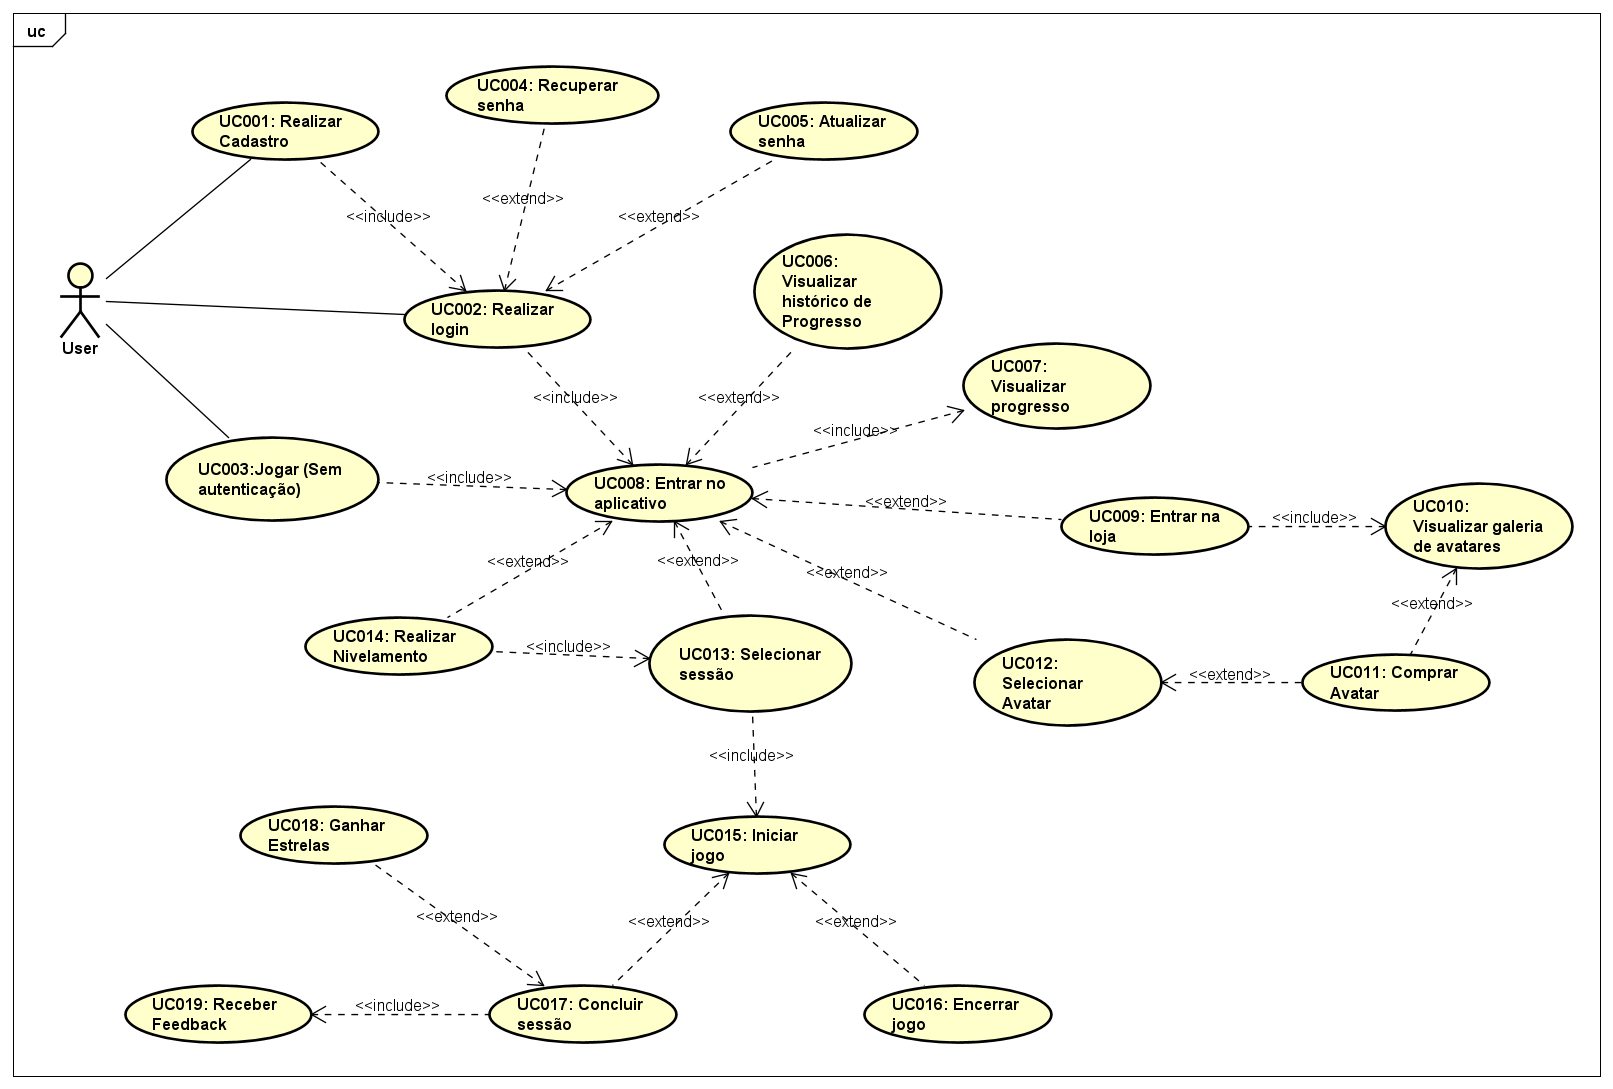
\includegraphics[width=\linewidth]{figuras/UseCase_TCC-1.png}
    \captionof{figure}{Diagrama de caso de uso Fonte: Autores}

    \label{fig:nome-da-imagem}
\end{center}
        \item \textbf{Diagrama de Classes}
        \item \textbf{Diagrama de Atividades}
    \end{itemize}
\end{itemize}

\section{Ferramentas e Tecnologias}

Na presente seção, serão detalhadas as diversas ferramentas e tecnologias empregadas na condução desta pesquisa, desempenhando um papel essencial na coleta, análise e desenvolvimento da pesquisa. A escolha criteriosa desses recursos é fundamental para a robustez e eficácia do estudo, proporcionando uma base sólida para a consecução dos objetivos propostos.

\begin{itemize}

    \item \textbf{React Native} 
    \begin{center}
    
\includegraphics[width=0.5\linewidth]{figuras/React Native.png}
    \captionof{figure}{Logo do framework React Native}
    \label{fig:React Native}
    Fonte para o React Native\footnote{\url{https://reactnative.dev/}}
\end{center}

O React Native é um framework de desenvolvimento de aplicativos móveis que permite a criação de aplicativos nativos para iOS e Android usando JavaScript e React.

A interface foi construída com componentes React Native, possibilitando alta reusabilidade e facilidade de manutenção. O gerenciamento de estado global foi feito via Context API e hooks. Para estilização, usou-se Styled Components com tematização adaptável. A lógica do jogo e regras foram implementadas em JavaScript puro. Atenção especial foi dada à acessibilidade e aspectos cognitivos do público-alvo. O código está organizado seguindo as melhores práticas de React, com componentes pequenos e funções puras. Para qualidade, adotou-se tipagem, testes unitários e integração contínua.No geral, a stack adotada demonstrou alta produtividade e capacidade de entregar uma experiência cross-platform de alto nível e alinhada às necessidades do projeto.

Sobre as versões utilizadas o projeto demonstra o desenvolvimento de um app React Native com recursos avançados de UI, navegação, mídia e animações. O uso do Expo simplifica o setup e configuração do ambiente de desenvolvimento. As versões recentes das principais dependências indicam que o projeto segue as melhores práticas para React Native. No geral, ilustrando um app mobile robusto e bem estruturado utilizando a biblioteca React Native e o ecossistema de ferramentas adjacentes. Utilizando a versão do react 18.2.0 e a versão do react native 0.71.3. 

    \item \textbf{React Native Voice}

    \begin{center}
    
\includegraphics[width=0.5\linewidth]{figuras/React Native Voice.png}
    \captionof{figure}{Logo biblioteca do React Native Voice}
    \label{fig:React Native Voice}
    Fonte para o React Native Voice\footnote{\url{https://github.com/react-native-voice/voice}}
\end{center}

A funcionalidade de reconhecimento de fala foi implementada através da biblioteca open-source react-native-voice, que provê uma API nativa para acesso às funcionalidades de speech-to-text do iOS e Android. A initialização acontece por meio da importação da biblioteca e chamada aos métodos Voice.start() e Voice.stop() para iniciar e interromper o reconhecimento, respectivamente. Configurou-se handlers para os eventos de início e fim da fala, além de tratamento do resultado do texto reconhecido em Voice.onSpeechResults. Após obter a transcrição, ela pode ser utilizada dentro da aplicação React Native, viabilizando diversos usos como entrada de texto por voz e comandos de voz. Optou-se por uma abordagem nativa por ser mais performatica e prover acesso direto às APIs específicas de cada plataforma. A implementação seguiu as melhores práticas recomendadas na documentação da biblioteca, garantindo robustez e experiência transparente entre Android e iOS.
    \item \textbf{Expo}
    \begin{center}
    
\includegraphics[width=0.5\linewidth]{figuras/Expo Framework.jpeg}
    \captionof{figure}{Logo do framework Expo}
    \label{fig:Expo}
    Fonte para o Expo Framework\footnote{\url{https://expo.dev/}}
\end{center}

O Expo é uma plataforma para simplificar o desenvolvimento de aplicativos móveis, especialmente em React Native. Ele oferece facilidade de configuração, desenvolvimento sem necessidade de compilação, bibliotecas prontas para uso e ferramentas como o Expo Client para testar aplicativos de forma rápida. O Expo é uma escolha popular para desenvolvedores que buscam uma abordagem simplificada e eficiente no desenvolvimento móvel.

    \item \textbf{Firebase}
    \begin{center}
    
\includegraphics[width=0.5\linewidth]{figuras/Firebase.png}
    \captionof{figure}{Logo do Firebase}
    \label{fig:Firebase}
    Fonte para o Firebase\footnote{\url{https://firebase.google.com/}}
\end{center}

O Firebase é uma plataforma de desenvolvimento de aplicativos da Google que oferece uma variedade de serviços prontos para uso, como autenticação, banco de dados em tempo real, armazenamento de arquivos, hospedagem e mensagens em nuvem. Ele simplifica o desenvolvimento, permitindo que os desenvolvedores integrem funcionalidades essenciais aos seus aplicativos sem a necessidade de configurar servidores complexos. O Firebase é conhecido por sua facilidade de uso e escalabilidade, sendo uma escolha popular para o desenvolvimento rápido de aplicativos web e móveis.

O Firebase fornece uma excelente plataforma de backend como serviço (BaaS) para o projeto. Ele permite o armazenamento de dados na nuvem em tempo real, autenticação de usuários, notificações push e análise de dados, entre outros recursos. Isso simplifica muito o desenvolvimento do aplicativo, pois lida com toda a infraestrutura do backend. Além disso, tem integração nativa com dispositivos Android e iOS, o que é ideal para este projeto mobile. Como o foco está na experiência de aprendizado gamificada, permite que a equipe se concentre na construção da melhor interface e jogabilidade sem se preocupar com complexidades de backend. Portanto, é uma excelente escolha como BaaS para este projeto educacional.
    \item \textbf{TypeScript}
    \begin{center}
    
\includegraphics[width=0.5\linewidth]{figuras/TypeScript.png}
    \captionof{figure}{Logo do TypeScript}
    \label{fig:TypeScript}
    Fonte para a documentação do TypeScript\footnote{\url{https://www.typescriptlang.org/docs/handbook/typescript-in-5-minutes.html}}
\end{center}

O TypeScript é uma linguagem de programação amplamente adotada no desenvolvimento de aplicativos web e mobile. Sua popularidade se deve ao fato de ser um superconjunto tipado do JavaScript, agregando segurança e produtividade à linguagem original. Quando combinado ao framework React Native, o TypeScript se mostra uma excelente escolha para projetos mobile.

Uma das principais vantagens de utilizá-lo com React Native é a capacidade de reaproveitar código entre plataformas. Como o TypeScript é compilado para JavaScript, linguagem nativa do React Native, os desenvolvedores conseguem compartilhar a maior parte do código entre iOS e Android. Isso aumenta a eficiência no desenvolvimento de apps multiplataforma.

Além disso, Typescript possui um vasto ecossistema de bibliotecas e frameworks, incluindo aqueles voltados para React Native. Essas ferramentas facilitam a implementação de recursos como animações, gerenciamento de estado e integração com APIs. A comunidade ativa contribui com tutoriais, documentações e fóruns de discussão, provendo amplo suporte ao desenvolvimento.

Ao optar pelo Typescript com React Native, os desenvolvedores garantem uma linguagem versátil e uma plataforma robusta para a criação de apps modernos e de alta qualidade. A união dessas tecnologias permite um fluxo ágil e produtivo, entregando ao usuário final uma experiência enriquecida. Portanto, o Typescript se consolida como uma ótima escolha para projetos mobile com React Native.

O projeto é um exemplo de aplicação das modernas práticas de desenvolvimento de software. Ele segue uma arquitetura modular, que permite uma maior facilidade de manutenção e extensão do código. O projeto é todo escrito em TypeScript, uma linguagem que oferece segurança de tipo e evita erros comuns em JavaScript.
Além disso conta com o apoio de diversas bibliotecas de terceiros, que fornecem funcionalidades adicionais, como gerenciamento de estado com Redux, roteamento com React Navigation, persistência de dados com AsyncStorage, entre outras. Para garantir a qualidade e a confiabilidade do código, o projeto possui uma suíte abrangente de testes, que utiliza ferramentas como Jest, Enzyme e Detox, facilitando o desenvolvimento e manutenção da aplicação em si.

Por que TypeScript?

    O TypeScript é uma variação do JavaScript que traz benefícios como:

    Tipagem Estática: Ajuda a evitar erros comuns, tornando o código mais claro.

    Melhoria na Segurança e Eficiência: O compilador pode detectar e corrigir erros de tipo em tempo de compilação, economizando tempo na depuração.

    Escalabilidade: Torna o código mais modular e reutilizável, melhorando a escalabilidade.

    \item \textbf{Astah UML}
    \begin{center}
    
\includegraphics[width=0.5\linewidth]{figuras/Astah UML.png}
    \captionof{figure}{logo da ferramenta para criação de UMLs AstahUML }
    \label{fig:Astah UML}
    Fonte para o AstahUML\footnote{\url{https://astah.net/products/astah-uml/}}
\end{center}

O Astah UML é uma ferramenta de modelagem UML (Unified Modeling Language) que oferece recursos abrangentes para profissionais de software, analistas de sistemas e outros envolvidos no desenvolvimento de software. Ele suporta todos os principais diagramas da UML, incluindo diagramas de classe, sequência, atividade, estado, e muito mais. Isso permite que os usuários visualizem e documentem diferentes aspectos de um sistema.
    \item \textbf{Figma}
    \begin{center}
    
\includegraphics[width=0.5\linewidth]{figuras/Figma.png}
    \captionof{figure}{logo da ferramenta de Design Figma}
    \label{fig:Figma}
    Fonte para o Figma Fonte\footnote{\url{https://www.figma.com/}}
\end{center}

O Figma é uma plataforma de design colaborativo baseada na web que revoluciona a maneira como equipes de design trabalham. Permitindo colaboração em tempo real, prototipagem interativa e a criação de bibliotecas de componentes reutilizáveis, o Figma oferece uma abordagem flexível e centrada na equipe para o design de interfaces de usuário (UI) e experiência do usuário (UX). Sua facilidade de uso, ampla compatibilidade com formatos de arquivo e integração fluida com outras ferramentas fazem dele uma escolha popular para profissionais de design e desenvolvimento em todo o mundo.

O Figma foi utilizado para diagramar os wireframes das principais telas e fluxos de navegação do aplicativo. Isso permitiu testar rapidamente como o usuário interage com os elementos de gamificação e conteúdos didáticos já neste estágio inicial. O wireflow desenvolvido no Figma serviu como guia para o desenvolvimento visual e codificação do aplicativo, garantindo que o produto final atendesse às necessidades dos usuários. O protótipo interativo criado também facilitou testes com usuários reais ainda nas fases iniciais do projeto e serviu como base para a evolução da aplicação, fornecendo feedback valioso antes de escrever qualquer linha de código a fim de validações. Seguimos o layout fornecido como base para a implementação. 

Os fluxos de navegação também ajudam a comunicar a jornada do usuário para a equipe, pois permitem visualizar o caminho que um usuário irá percorrer ao realizar determinadas ações. A combinação de wireframes e fluxos de navegação no Figma torna a prototipação uma etapa crucial no processo de design, permitindo uma melhor compreensão das interações e proporcionando uma base sólida para o desenvolvimento do produto.
   
\end{itemize}

\section{Prototipação de telas}

A prototipação de telas é uma etapa importante no design de aplicativos e sites, que permite simular a experiência do usuário antes mesmo de construir o produto final. O protótipo consiste em um modelo interativo das telas, contendo os fluxos de navegação e os elementos de interface. Ele pode ter diferentes níveis de fidelidade, desde esboçosSimples até designs mais refinados. 

A grande vantagem da prototipação é permitir testar e validar ideias de forma rápida e barata, identificando problemas na experiência do usuário precocemente, antes de partir para a programação. Ferramentas como Figma, Adobe XD e Proto.io facilitam a criação de protótipos clicáveis que simulam os comportamentos da interface. Com testes iterativos envolvendo usuários reais, o protótipo é aprimorado até chegar em um design pronto para ser desenvolvido. Dessa forma, a prototipação ajuda a economizar tempo e evitar retrabalho no processo de design.

\subsection{Desenvolvimento do protótipo}


\begin{itemize}
    \item \textbf{Participantes e procedimentos da avaliação do protótipo}
    \item \textbf{Validação: testes de usabilidade, observação de uso, feedback dos usuários}
    
\end{itemize}

\section{Repositório}

O que é um Repositório?

Um repositório no GitHub é como um cofre para seu projeto. Ele contém todos os arquivos do seu projeto, além do histórico de todas as alterações feitas ao longo do tempo. É como uma versão online do seu projeto que facilita a colaboração e o controle de versões.

Estrutura do Repositório

Branches

No contexto do GitHub, usamos "branches" para criar diferentes versões do projeto. Cada branch é uma ramificação independente do código-fonte, possibilitando que você isole e desenvolva novas funcionalidades, refatore o código ou faça correções e testes em paralelo, sem interferir no código existente na branch principal, que geralmente é nomeada como \textit{main} \cite{al}. Neste projeto, utilizamos apenas a branche \textit{main}.


Refatoração e Aprimoramento

Uma análise crítica da estrutura existente levou a mudanças significativas. A reestruturação do código, adotando melhores práticas e aprimorando a arquitetura. Bem como a criação de uma nova branche nomeada de develop ...................

E o projeto ficou organizado da seguinte maneira: 

Branche main

............

Branche develop

..............

Versionamento do Código

Versão 0.0.1 -  Criação do projeto.

Versão 0.1.0 - Organizamos as pastas de forma mais lógica. Cada tipo de funcionalidade agora tem seu próprio espaço. Para facilitar a compreensão e manutenção do código.

Versão 0.2.0 - Componentização. Dividimos os componentes em partes menores, cada uma realizando uma tarefa específica. Isso ajuda na organização e na compreensão do código.

Versão 0.3.0 - Separamos os arquivos de estilo, proporcionando uma consistência visual melhor.

Versão 0.4.0 - Movemos o gerenciamento de estado para "stores", proporcionando uma prática recomendada para projetos React Native.

Versão 1.0.0-alpha - Decidimos mudar a tecnologia utilizada de JavaScript para TypeScript.


Onde usar??  ->  Essas mudanças visavam criar uma base de código mais organizada, fácil de entender e pronta para receber atualizações e melhorias no futuro. Este projeto, agora utilizando TypeScript e seguindo melhores práticas, está mais preparado para crescer de maneira sustentável e com qualidade.


        
  % Texto do cap4.tex
\chapter{Experimento e Coleta de Dados}\label{chp:exp}




\section{Análise da Matriz Curricular do Ensino Fundamental 1 (4º Ano) na Matéria de Matemática}

A análise da matriz curricular do Ensino Fundamental 1, especificamente para o 4º ano na matéria de Matemática, envolve a comparação entre o conteúdo programático do Colégio Salesiano do Salvador e o Referencial Curricular Municipal de Salvador. Ambos os documentos têm como objetivo proporcionar uma educação matemática abrangente, mas diferem em sua abordagem e detalhamento.

\item \textbf{Conteúdo Programático do Colégio Salesiano do Salvador}

 No Colégio Salesiano do Salvador, o currículo de Matemática para o 4º ano é dividido em três trimestres, cada um abordando tópicos específicos. No primeiro trimestre, os alunos são introduzidos aos números romanos e ao sistema de numeração decimal na base 10, com foco em números até a dezena de milhar. Além disso, há uma ênfase na composição e decomposição de números, valor posicional, arredondamento e estimativa. 

Durante o segundo trimestre, o currículo avança para multiplicação e divisão, introduzindo conceitos como múltiplos, propriedades da multiplicação e divisão por 10, 100 e 1000. A geometria é também abordada, com os alunos aprendendo sobre perímetro e a ideia de área. Estatística e probabilidade são introduzidas, com foco em variáveis categóricas e numéricas e na criação e interpretação de tabelas e gráficos.

No terceiro trimestre, o currículo foca em números decimais, abordando sua utilização no sistema monetário brasileiro, bem como adição e subtração de números decimais. Geometria continua a ser explorada, incluindo conceitos de ângulos (retos, agudos e obtusos), retas paralelas e perpendiculares, simetria, prismas e pirâmides. A educação financeira é introduzida, ensinando conceitos de consumo, valores de vida e empreendedorismo. \cite{conteudo_programatico_salesiano}

\item \textbf{Referencial Curricular Municipal de Salvador}

O Referencial Curricular Municipal para os anos iniciais do ensino fundamental de Salvador apresenta uma abordagem integrada e contínua para a aprendizagem matemática. Este currículo também abrange números e operações, geometria, grandezas e medidas, e tratamento da informação, mas com uma estrutura menos fragmentada por trimestre.

Os alunos são incentivados a resolver problemas que envolvem adição, subtração, multiplicação e divisão com números naturais, além de realizar diferentes tipos de cálculos (exatos, aproximados e mentais). A geometria é integrada ao aprendizado diário, com foco na identificação, descrição e representação da localização e movimentação de objetos no espaço, bem como na análise e comparação de figuras geométricas planas e espaciais.

Grandezas e medidas são abordadas através da resolução de problemas que envolvem a estimativa e medição de diferentes quantidades, como tempo, comprimento, massa e capacidade. Os alunos aprendem a utilizar medidas de tempo e a realizar conversões simples, além de aplicar esses conceitos em situações práticas.

O tratamento da informação é enfatizado com a coleta e interpretação de dados, apresentando resultados em tabelas e gráficos de colunas. Os alunos são ensinados a coletar dados de duas variáveis, a criar tabelas e gráficos simples e de dupla entrada, e a interpretar as informações apresentadas. 
\cite{referencial_curricular_municipal}


\section{Comparação entre Matrizes de Ensino: Temas e Abordagens Principais}

Comparando os dois currículos, foi observado que ambos cobrem os principais tópicos de Matemática necessários para o 4º ano, mas com diferenças notáveis em sua abordagem. O currículo do Colégio Salesiano do Salvador é mais detalhado e dividido claramente por trimestres, oferecendo uma estrutura bem definida para cada período letivo. Em contraste, o Referencial Curricular Municipal de Salvador adota uma abordagem mais integrada, com foco na aplicação prática dos conhecimentos e na resolução de problemas contínua ao longo do ano.

A inclusão de educação financeira no currículo do Colégio Salesiano é um diferencial, pois aborda aspectos como consumo, valores de vida e empreendedorismo, preparando os alunos para lidar com questões financeiras desde cedo. Por outro lado, o Referencial Curricular Municipal de Salvador enfatiza a interpretação de dados e a aplicação prática dos conceitos matemáticos, promovendo uma compreensão mais ampla e contextualizada da matemática no dia a dia dos alunos.

Ambos os currículos são eficazes em seus objetivos, oferecendo uma educação matemática completa e adequada para os alunos do 4º ano, mas com metodologias e enfoques distintos que refletem suas respectivas filosofias educacionais.

\begin{longtable}{|>{\raggedright}p{3cm}|>{\raggedright}p{6cm}|>{\raggedright}p{6cm}|}
\hline
\textbf{Tópicos} & \textbf{Colégio Salesiano do Salvador} & \textbf{Referencial Curricular Municipal de Salvador} \\
\hline
Números e Operações & Números romanos, sistema de numeração decimal, números até dezena de milhar, adição, subtração, multiplicação, divisão & Relações subjacentes a números, operações com números naturais, cálculos exatos, aproximados e mentais \\
\hline
Geometria & Perímetro, área, ângulos, retas paralelas e perpendiculares, prismas, pirâmides, simetria & Localização e movimentação de objetos, figuras geométricas planas e espaciais, ângulos retos e não retos \\
\hline
Estatística e Probabilidade & Variáveis categóricas e numéricas, tabelas, gráficos, gráfico pictórico & Estimativa e medição de tempo, comprimento, massa, capacidade, conversões simples \\
\hline
Grandezas e Medidas & Medidas de comprimento, massa, capacidade, tempo, temperatura & Estimativa de diferentes medidas, medições efetivas, uso de medidas de tempo \\
\hline
Educação Financeira & Consumo, valores de vida, crenças, paradigmas, aposentadoria, proteção, empreendedorismo, metas, cooperativismo, renda e consumo & Não especificado \\
\hline
Tratamento da Informação & Coleta de dados, apresentação em tabelas e gráficos & Coleta e interpretação de dados, criação de tabelas e gráficos simples e de dupla entrada \\
\hline

\caption{Tabela comparativa entre matrizes curriculares de matemática básica do ensino fundamental 1, 4º ano}
\end{longtable}

\section{Estruturação e Acompanhamento dos Temas Abordados na Aplicação}


Para enriquecer essa análise, utilizou-se o Khan Academy como uma base de dados para coleta de assuntos, garantindo uma abordagem ampla e atualizada dos tópicos. Baseada no conteúdo programático anterior chegamos ao filtro do conteúdo programático mais relevantes para a aplicação com base nesse estudo. A plataforma fornece uma vasta gama de materiais educativos, exercícios práticos e vídeos explicativos que cobrem os tópicos abordados nas matrizes curriculares. \cite{khanacademy_numeros_soma_subtracao}

\begin{longtable}{|>{\raggedright}p{2cm}|>{\raggedright}p{4cm}|>{\raggedright}p{4cm}|>{\raggedright}p{4cm}|}
\hline
\textbf{Unidade} & \textbf{Tópicos no Khan Academy} & \textbf{Colégio Salesiano do Salvador} & \textbf{Referencial Curricular Municipal do Salvador} \\
\hline
Unidade 1 & Números: soma e subtração & Adição, subtração, propriedades da adição, expressões numéricas, situações-problema & Relações subjacentes a números, operações com números naturais, cálculos exatos, aproximados e mentais \\
\hline
Unidade 2 & Números: multiplicação e divisão & Multiplicação, divisão, propriedades da multiplicação, regularidades da divisão, situações-problema & Relações subjacentes a números, operações com números naturais, cálculos exatos, aproximados e mentais \\
\hline
Unidade 3 & Números: frações & Não especificado & Noção de fração, leitura de fração, comparação de frações, adição e subtração de frações, situações-problema \\
\hline
Unidade 4 & Álgebra & Não especificado & Noção de equação, valor desconhecido, relações de igualdade, operações inversas \\
\hline
Unidade 5 & Geometria & Perímetro, área, ângulos, retas paralelas e perpendiculares, prismas, pirâmides, simetria & Localização e movimentação de objetos, figuras geométricas planas e espaciais, ângulos retos e não retos \\
\hline
Unidade 6 & Grandezas e medidas & Medidas de comprimento, massa, capacidade, tempo, temperatura & Estimativa de diferentes medidas, medições efetivas, uso de medidas de tempo \\
\hline
Unidade 7 & Probabilidade e estatística & Variáveis categóricas e numéricas, tabelas, gráficos, gráfico pictórico & Coleta e interpretação de dados, criação de tabelas e gráficos simples e de dupla entrada \\
\hline
Unidade 8 & Educação financeira & Consumo, valores de vida, crenças, paradigmas, aposentadoria, proteção, empreendedorismo, metas, cooperativismo, renda e consumo & Não especificado \\
\hline

\caption{Tabela De Assuntos Para Estruturação E Acompanhamento}

\end{longtable}


\section{Formulário abordado}

A ideia é coletar feedback sobre um protótipo de aplicativo gamificado que tem como objetivo auxiliar professores no ensino de matemática básica para alunos do ensino fundamental I. O formulário de avaliação é composto por várias seções que buscam abordar diferentes aspectos do aplicativo, desde a usabilidade e design visual até a efetividade das ferramentas disponíveis e o engajamento dos alunos. Os dados coletados serão usados para ajustar o aplicativo de acordo com as necessidades reais, melhorar continuamente a experiência do usuário e validar as hipóteses iniciais sobre a efetividade do aplicativo na promoção do ensino de matemática básica. 

\subsection{Analise das perguntas do formulário Gamificação como Estratégia para o Ensino de Matemática Básica para Alunos do Ensino Fundamental I}

Com base no estudo em questão elaboramos esse questionário com algumas perguntas chaves para a validação com os professores tendo os seguintes questionamentos para facilitar o entendimento utlizamos um video com o protótipo em questão: 


\begin{enumerate}[label=\arabic*.]
    \item \textbf{Você acha que atividades gamificadas estimulam o interesse e o engajamento dos alunos?}
    \begin{itemize}
        \item \textbf{Respostas possíveis}: Sim / Não
        \item \textbf{Objetivo}: Avaliar se os professores acreditam que a gamificação é uma estratégia eficaz para aumentar o interesse e o engajamento dos alunos no ensino de matemática.
    \end{itemize}
    
    \item \textbf{As funcionalidades do aplicativo (desafios, recompensas) são eficazes para o aprendizado de matemática?}
    \begin{itemize}
        \item \textbf{Respostas possíveis}: Sim / Não
        \item \textbf{Objetivo}: Medir a percepção dos professores sobre a eficácia das funcionalidades gamificadas (como desafios e recompensas) no aprendizado de matemática.
    \end{itemize}
    
    \item \textbf{Você sentiu falta de alguma funcionalidade que acha crucial para a ideia da aplicação?}
    \begin{itemize}
        \item \textbf{Respostas possíveis}: Sim / Não
        \item \textbf{Objetivo}: Identificar se os professores percebem a ausência de alguma funcionalidade importante que poderia melhorar a aplicação.
    \end{itemize}
    
    \item \textbf{Se a sua última resposta foi Sim, diga qual funcionalidade gostaria na aplicação.}
    \begin{itemize}
        \item \textbf{Respostas abertas}
        \item \textbf{Objetivo}: Coletar sugestões específicas de funcionalidades que poderiam ser adicionadas para melhorar a aplicação.
    \end{itemize}
\end{enumerate}

\subsection{Sessões das Telas da Aplicação}

\begin{enumerate}[label=\arabic*.]
    \item \textbf{O aplicativo oferece recursos que complementam e contribuem com o ensino em sala de aula?}
    \begin{itemize}
        \item \textbf{Respostas possíveis}: Sim / Não
        \item \textbf{Objetivo}: Verificar se o aplicativo é visto como uma ferramenta complementar eficaz para o ensino em sala de aula.
    \end{itemize}
    
    \item \textbf{A interface do aplicativo é visivelmente fácil de navegar?}
    \begin{itemize}
        \item \textbf{Respostas possíveis}: Sim / Não
        \item \textbf{Objetivo}: Avaliar a usabilidade da interface do aplicativo, garantindo que ela seja fácil de navegar para os usuários.
    \end{itemize}
    
    \item \textbf{As instruções e informações estão claras e concisas?}
    \begin{itemize}
        \item \textbf{Respostas possíveis}: Sim / Não
        \item \textbf{Objetivo}: Verificar se as instruções e informações fornecidas no aplicativo são claras e compreensíveis.
    \end{itemize}
    
    \item \textbf{Os elementos visuais (cores, fontes, imagens) são adequados para o público-alvo?}
    \begin{itemize}
        \item \textbf{Respostas possíveis}: Sim / Não
        \item \textbf{Objetivo}: Avaliar a adequação dos elementos visuais do aplicativo para os alunos do ensino fundamental I.
    \end{itemize}
    
    \item \textbf{As telas apresentam elementos de gamificação?}
    \begin{itemize}
        \item \textbf{Respostas possíveis}: Sim / Não
        \item \textbf{Objetivo}: Confirmar a presença de elementos de gamificação nas telas do aplicativo.
    \end{itemize}
    
    \item \textbf{As telas estão visualmente atraentes?}
    \begin{itemize}
        \item \textbf{Respostas possíveis}: Sim / Não
        \item \textbf{Objetivo}: Avaliar a atratividade visual das telas do aplicativo.
    \end{itemize}
    
    \item \textbf{Você tem alguma sugestão para melhorar o design ou a organização das telas?}
    \begin{itemize}
        \item \textbf{Respostas possíveis}: Sim / Não
        \item \textbf{Objetivo}: Coletar sugestões sobre possíveis melhorias no design ou na organização das telas do aplicativo.
    \end{itemize}
\end{enumerate}

\subsection{Conteúdo e Atividades}

\begin{enumerate}[label=\arabic*.]
    \item \textbf{Os assuntos abordados são condizentes com o público-alvo?}
    \begin{itemize}
        \item \textbf{Respostas possíveis}: Sim / Não
        \item \textbf{Objetivo}: Verificar se os conteúdos abordados no aplicativo são apropriados para os alunos do ensino fundamental I.
    \end{itemize}
    
    \item \textbf{O plano de atividades proposto é válido para este público?}
    \begin{itemize}
        \item \textbf{Respostas possíveis}: Sim / Não
        \item \textbf{Objetivo}: Avaliar a adequação do plano de atividades para o público-alvo.
    \end{itemize}
\end{enumerate}

\subsection{Avaliação Geral}

\begin{enumerate}[label=\arabic*.]
    \item \textbf{Se aplicável, você consideraria utilizar o aplicativo como parte de atividades educacionais?}
    \begin{itemize}
        \item \textbf{Respostas possíveis}: Sim / Não
        \item \textbf{Objetivo}: Identificar a disposição dos professores em utilizar o aplicativo em suas atividades educacionais.
    \end{itemize}
    
    \item \textbf{Como profissional da área, qual é a sua impressão geral sobre o aplicativo?}
    \begin{itemize}
        \item \textbf{Resposta aberta}
        \item \textbf{Objetivo}: Coletar uma impressão geral dos professores sobre o aplicativo.
    \end{itemize}
    
    \item \textbf{Você possui alguma observação ou sugestão adicional que não foi mencionada nas avaliações anteriores?}
    \begin{itemize}
        \item \textbf{Resposta aberta}
        \item \textbf{Objetivo}: Permitir que os professores adicionem quaisquer outras observações ou sugestões que considerem relevantes.
    \end{itemize}
    
    \item \textbf{Você acha que o aplicativo seria fácil de implementar em sua rotina de ensino?}
    \begin{itemize}
        \item \textbf{Respostas possíveis}: Sim / Não
        \item \textbf{Objetivo}: Avaliar a facilidade de implementação do aplicativo na rotina de ensino dos professores.
    \end{itemize}
    
    \item \textbf{Em sua opinião, quais os pontos fortes e fracos deste aplicativo?}
    \begin{itemize}
        \item \textbf{Resposta aberta}
        \item \textbf{Objetivo}: Identificar os pontos fortes e fracos do aplicativo segundo a percepção dos professores.
    \end{itemize}
    
    \item \textbf{Que nota você daria ao aplicativo em uma escala de 0 a 10?}
    \begin{itemize}
        \item \textbf{Resposta numérica}
        \item \textbf{Objetivo}: Obter uma avaliação quantitativa geral do aplicativo.
    \end{itemize}
\end{enumerate}



 % Texto do cap5.tex
\chapter{Conclusões}\label{chp:conc}

Concluímos que a evolução do aplicação ocorreu de forma fluída e assertiva, captando os principais pontos que faltavam na aplicação como a perssistencia de dados, login do usuário, alimentar mais sessões para progressão de fases. 

O desenvolvimento desta idealização e estudo de negócio para o ensino de matemática de forma lúdica e acessível para crianças coms revelou pontos positivos e oportunidades de melhoria. A abordagem em formato de jogo se mostrou engajadora, permitindo praticar os conceitos de forma motivadora. A incorporação de funcionalidades como reconhecimento de voz também trouxe benefícios de independência e confiança.

Porém, ficou evidente que alguns ajustes são necessários. É preciso expandir o conteúdo abordado e níveis de dificuldade, para cobrir de forma mais completa o currículo matemático adaptado. A adaptação da linguagem e representação visual aos diferentes estágios cognitivos do público-alvo também é essencial. E a gamificação poderia ser aprimorada com mecânicas mais sólidas de progressão e recompensa.

No geral, o projeto mostrou o potencial da tecnologia para promover o ensino inclusivo e personalizado para crianças com necessidades especiais. Mas requer continuidade, com base no aprendizado obtido nesta primeira versão. A equipe está motivada a seguir evoluindo a solução e explorando novas possibilidades.


Em conclusão, este projeto representa apenas o primeiro passo de uma trajetória. Há ainda muito trabalho para que a tecnologia educacional seja de fato inclusiva e acesse todo o seu potencial transformador. Mas com a continuidade certa, temos a convicção de estar no caminho para tornar o ensino mais igualitário e efetivo para todos.



\section{Trabalhos futuros}

Como trabalhos futuros deixaremos como sugestiva o aprimoramento da aplicação, utilizando sessões e a implementação de uma inteligência artificial para o nívelamente mais assertivo e nível de dificuldade para a criança que interagir com o aplicativo. 



z % Texto do cap6.tex



%%%%%%%%%%%%%%%%%%%%%%%%%%
%%Elementos Pós-Textuais%%
%%%%%%%%%%%%%%%%%%%%%%%%%%
%%--------Bibliografia--------
\Bibliografia{referenciasbibliograficas} % arquivo bibtex com as referências (referenciasbibliograficas.bib)

\cite{furlan2016desenvolvimento}

%%--------Apêndice--------
%% Descomente caso exista a necessidade da inclusão de apêndices
%\apendice % Comando que inclui os apêndices
%\include{7_Apendice/apendice_1}   % Arquivo apendice_1.tex
%\include{7_Apendice/apendice_2}   % Arquivo apendice_2.tex
%%---------------------------------------------------------------

%%--------Anexos-------------------------------------------------
%% Descomente caso exista a necessidade da inclusão de anexos
%\anexo % Comando que inclui os anexos (outros autores)
%\include{8_Anexos/anexo_1}  % Arquivo anexo_1.tex
%\include{8_Anexos/anexo_2}  % Arquivo anexo_2.tex
%%---------------------------------------------------------------
\appendix


\chapter{Apêndice}

\begin{figure}
  \centering
  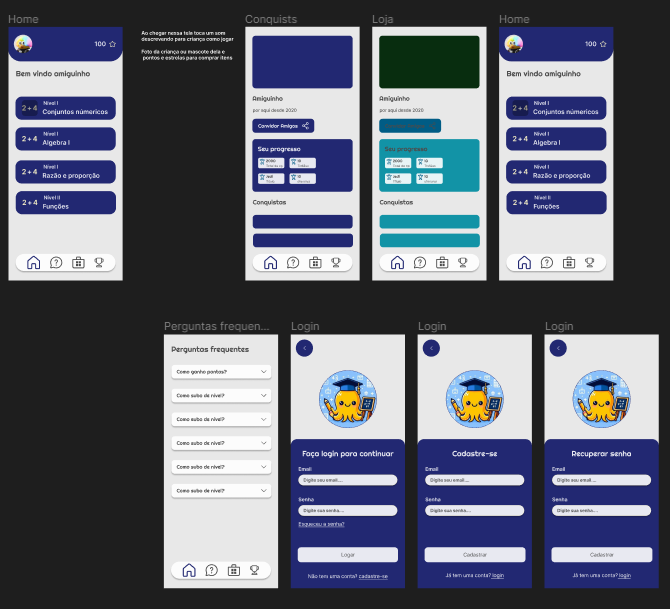
\includegraphics[width=\linewidth]{figuras/T21.png}
  \caption{Prototipação de telas: Autoral desenvolvida pela equipe T21, 2023.}
  \label{fig:nome-da-imagem}
\end{figure}

\begin{center}
    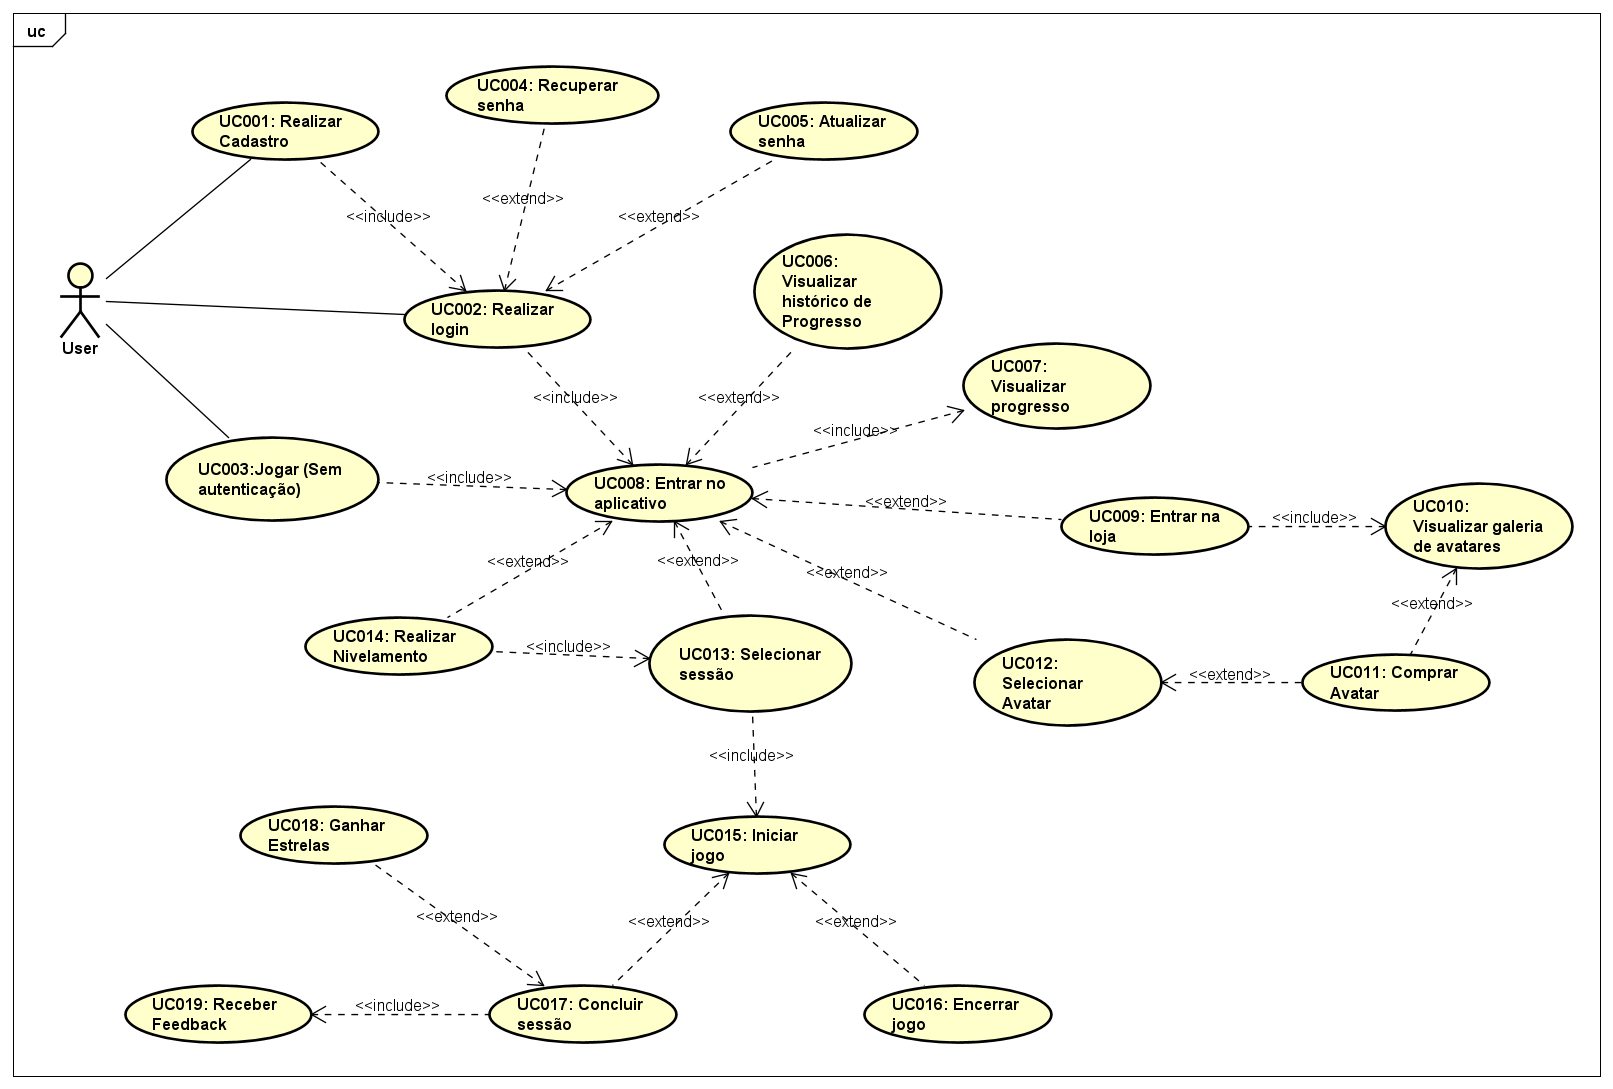
\includegraphics[width=\linewidth]{figuras/UseCase_TCC-1.png}
    \captionof{figure}{Diagrama de caso de uso - Requisitos Funcionais: Autoral desenvolvida pela equipe, 2023.}
    \label{fig:nome-da-imagem}
\end{center}


\end{document}
